\chapter[Notions fondamentales en \textsc{Python}]{Notions fondamentales}
\label{chap:X}

%%%--- Note de rédaction
%%%--- Pour bien distinguer les différentes manières d'utiliser l'interpréteur
%%%--- Python, ce chapitre n'utilise pas l'extension PythonTeX, mais des
%%%--- environnements dédiés de listings, de codes ou de terminaux.
%%%--- PythonTeX et sa présentation sous IDLE sont utilisés à partir de la 
%%%--- dernière section de ce chapitre (contrairement au MOOC.


\lettrine[findent=-0.7pt]{D}{epuis l'aube du millénaire, \textsc{Python} s'est imposé} comme un langage privilégié de programmation --- notamment avec la version 2.0 datant de 2000 ---, tout d'abord et faisant suite\parnote{Par exemple, la distribution \textsc{Ubuntu} adopte \textsc{Python} pour ses codes de configuration et « \emph{applets} » (petites applications) dès sa première version d'avril 2004, mais également, la plupart des logiciels libres majeurs (\textsc{Gimp}, \textsc{Inkscape}, etc.) proposent rapidement la possibilité de développer des greffons --- \emph{plug-ins} en anglais --- complémentaires à leur noyau principal, voire sont dans leur entièreté directement codés  en \textsc{Python}.} au domaine de l'informatique, en contexte universitaire et de recherche puis, au fur et à mesure de la notoriété grandissante de ses qualités, en tant qu'outil d'apprentissage et de formation à la programmation informatique : universités, écoles d'ingénieurs et désormais enseignement secondaire.
\parnotes

Les atouts intrinsèques de \textsc{Python} qui peuvent expliquer ce constat sont relatifs aux faits que c'est un langage interprété --- dit de \textit{script}, autrement dit sans étape de compilation --- que, par conception, sa syntaxe est dirigée par la lisibilité comme la facilité d'accès pour l'utilisateur, que c'est un langage de programmation orientée objet (\textsc{Poo}), qu'il est disponible pour tout système d'exploitation --- \textsc{Windows}, \textsc{MacOS} et \textsc{Linux} --- et enfin, non des moindres, que sa licence de diffusion est libre, y compris pour des applications à vocation commerciale.

Si dans ce \textsc{Mooc} et par conséquent ce document, l'acceptation originelle de \textsc{Python} par la communauté scientifique est abordée au moyen d'illustrations concrètes de son utilisation (voir \Cref{part:IV}, \qnameref{part:IV}), son volet pédagogique en est bien entendu la motivation essentielle et le propos principal : ne pas mettre la charrue avant ses fameux bœufs... 

% dans certains domaines d'application
 
%----------
\section[Écosystème et environnement]{Écosystème et environnement \textsc{Python}}
\label{sec:X.1}

Cette approche consacrée à \textsc{Python 3} --- à savoir que la version 2 du langage\sidenote{Actuellement en version 2.7 et définitivement figée sans autre révision.} a été plusieurs fois prorogée en coexistence avec la version 3 pour atteindre un basculement arrêté en 2020 --- débute par les présentation et mise en œuvre d'un environnement de travail fonctionnel.% cadre et opérationnel.

Sont ainsi évoqués en premiers lieux les généralités, l'organisation du matériel pédagogique puis les outils qui sont nécessaires de configurer pour la programmation avec \textsc{Python}.
La référence adoptée pour ce document, les exemples et exercices, est la version 3.6 de \textsc{Python}.

\subsection[Organisation du cours]{Organisation du \textsc{Mooc}}
\label{sub:X.1.1}

\begin{marginvideo}
	[\label{vid:X.1}Organisation du cours.]%
	%\href{./Videos/Chapter09/vidIX-01-organisation-HD.mp4}%
	%	{
\includegraphics[width=\marginparwidth]{./Images/Pictograms/film-strip-dark-electric-blue.png}}
	\movie[width=\marginparwidth,showcontrols]%
		{
\includegraphics[width=\marginparwidth]{./Images/Pictograms/film-strip-dark-electric-blue.png}}%
		{./Videos/Chapter10/vidX-01-organisation-HD.mp4}%
	\launchvideo{./Videos/Chapter10/vidX-01-organisation-HD.mp4}
\end{marginvideo}

En termes de contenus et d'organisation, ce \textsc{Mooc} se présente en deuxième édition. La mouture actuelle fait en effet suite à l'apprentissage de \textsc{Python} proposé entre 2014 et 2016, qui se fondait alors sur la version 2.7 du langage. Entre-temps, l'écosystème \textsc{Python} a largement versé en version 3 --- noyau comme multiples bibliothèques applicatives associées ou, selon le terme consacré, modules.

\subsubsection[Présentation]{Présentation}
\label{subsub:X.1.1.1}

L'exposé\sidenote{La partie sur \textsc{Python} du manuel est extraite du \textsc{Mooc} « \textsc{Python} :des fondamentaux aux concepts avancés du langage » et ne reprend que les deux premières semaines du tronc commun.} est articulé autour de deux grandes parties : un tronc commun réparti sur six semaines de travail et couvrant les fondamentaux d'apprentissage de \textsc{Python} puis, de manière optionnelle, quelques approfondissements correspondant à des utilisations spécifiques de \textsc{Python} et certains modules particuliers.

En terme de tronc commun, l'objectif est d'aborder les fondamentaux du langage, c'est-à-dire les types de base, les fonctions, les structures de contrôle, les modules, les espaces de nommage et la programmation objet. 
On insistera sur les traits marquants de \textsc{Python}, à savoir :
\begin{itemize}
	\item un langage très lisible ;
	\item pour lequel tout est objet ;
	\item qui, pour permettre une bonne compréhension du code, est associé à la notion de liaison lexicale mais également à celle de typage dynamique ;
	\item et dont l'approche serait incomplète sans parler des itérations et des espaces de nommage.
\end{itemize}

\sidegraphic{
\includegraphics[width=0.5\linewidth]{./Images/Chapter10/python-powered.png}}%
En ce qui concerne la partie optionnelle, trois directions sont proposées pour approfondir le cours de base. Une première semaine consacrée aux outils dits de «~\textit{data science}~», une deuxième pour aborder la «~programmation asynchrone~» --- sujet très innovant et très intéressant que vous êtes convié à consulter ---, puis enfin, en dernière semaine, un complément sur les « sujets avancés », à savoir l'approche des métaclasses, des décorateurs et des techniques de programmation qui n'ont pas été jugés utiles d'inclure au tronc commun.

Il est nécessaire de mentionner que des deux premières semaines ad\-ditionnelles proposées, il serait possible sans aucun problème de conduire un MOOC à part entière. Il s'agit donc d'une toute petite introduction pour savoir que cela existe et susciter suffisamment d'intérêt pour gratter au-delà de la surface et fournir les moyens d'approfondir tous ces sujets en autonomie.

Que les modules optionnels soient suivis ou non, l'enjeu est bien entendu de posséder le bagage nécessaire pour écrire du code propre, mais également de lire celui d'autres programmeurs. C'est un peu com\-me une langue étrangère, sans la lecture de code, on n'apprend pas les différents paradigmes et idiomes. C'est pour cette raison que, parfois, les informations données vont au-delà du strict nécessaire.  

Par ailleurs, la perspective est également de pouvoir choisir et utiliser à bon escient les bibliothèques tierces de l'écosystème \textsc{Python}. Un des atouts majeurs de \textsc{Python} est sa polyvalence.

En termes de linguistique, évidemment le propos est en français, ainsi que les exercices et les supports pédagogiques. Néanmoins, il est fait appel de nombreuses fois à des documents en anglais, pour la raison que le langage et, plus généralement, les documentations et la quasi intégralité des codes existants sont en anglais. 

En outre, certains termes sont parfois impossibles à traduire. Il a été convenu de conserver leur expression anglophone, permettant aussi, dès le départ, une recherche sur les moteurs de recherche plus aisée.


\subsubsection[Pourquoi \textsc{Python} ?]{Pourquoi \textsc{Python} ?}
\label{subsub:X.1.1.2}

\begin{marginvideo}
	[\label{vid:X.2}Choix de \textsc{Python}.]%
	%\href{./Videos/Chapter09/vidIX-02-pourquoipython-HD.mp4}%
	%	{
\includegraphics[width=\marginparwidth]{./Images/Pictograms/film-strip-dark-electric-blue.png}}
	\movie[width=\marginparwidth,showcontrols]%
		{
\includegraphics[width=\marginparwidth]{./Images/Pictograms/film-strip-dark-electric-blue.png}}%
		{./Videos/Chapter10/vidX-02-pourquoipython-HD.mp4}%
	\launchvideo{./Videos/Chapter10/vidX-02-pourquoipython-HD.mp4}
\end{marginvideo}

Avant de rentrer à proprement parler dans la technique, quelques mots sur les raisons qui expliquent que \textsc{Python} soit un langage très agréable à utiliser et qui peut servir à de nombreuses d'applications. 

\textsc{Python} possède une foultitude de bonnes propriétés dont à l'usage la principale : la lisibilité. Pour s'en convaincre, on peut conduire un comparatif avec un certain nombre d'autres langages généralistes. À titre uniquement indicatif, ce parallèle est conduit avec les langages de programmation \textsc{C++}, \textsc{Java} et \textsc{JavaScript}.


\overparagraph{Comparaison entre langages de programmation}

Si l'on compare la manière de construire une boucle sur une liste en \textsc{C++} et en \textsc{Python}, cela peut ressembler aux codes \ref{lst:X.1}. 

En \textsc{Python}, le code est déjà beaucoup plus court, moins touffu et il n'y a pratiquement aucun sucre syntaxique : pas de \texttt{begin}, de \texttt{end}, d'accolades et autres choses du même acabit.

En fait, le langage a pris le parti d'avoir une syntaxe orientée sur la présentation. Les deux phrases \texttt{print} et \texttt{manage} font partie du même bloc. L'œil humain le capte immédiatement, il n'y a pas besoin de rajouter des accolades ou des séparateurs du même genre.

La première chose importante à noter est donc que \textit{\textsc{Python} possède une syntaxe articulée sur la présentation}.

\begin{jazzcode*}
\caption{\label{lst:X.1}Comparaison d'une boucle réalisée en \textsc{C++} et en \textsc{Python}.}
%\captionof{listing}{\label{lst:X.1}Comparaison d'une boucle réalisée en \textsc{C++} et en \textsc{Python}.}
%\caption{\label{lst:X.1.a}Codage d'une boucle en \textsc{C++}}
%\caption{\label{lst:X.1.a}Codage d'une boucle en \textsc{Python}}
\begin{codebox}[width=0.665\linewidth, nobeforeafter]{cpp}
// parcourir une liste

for (Cell *cell = cells.start; cell != NULL; cell = cell.next) {
	print(cell);
	manage(cell);
}
\end{codebox}
\qquad\quad %\hfill
\begin{codebox}[width=0.265\linewidth, nobeforeafter]{python}
# parcourir une liste

for cell in cells:
	print(cell)
	manage(cell)
\end{codebox}
\end{jazzcode*}

%(cf. \cref{lst:X.2})

La deuxième comparaison est conduite avec le langage \textsc{Java}. L'exem\-ple pris ici est totalement pathologique ; un programme simple qui affiche « \textit{Hello, world!} » que l'on trouve dans toutes les introductions des livres de programmation.

\begin{jazzcode*}
\caption{\label{lst:X.2}Comparaison d'un programme « \emph{Hello world!} » en \textsc{Java} et en \textsc{Python}.}
\begin{codebox}[width=0.45\linewidth, nobeforeafter]{java}
public class HelloWorld
{
	public static void main (string[] args)
	{
		System.out.println("Hello world!");
	}
}
\end{codebox}
\qquad\quad %\hfill
\begin{codebox}[width=0.265\linewidth, nobeforeafter]{python}
print("Hello world!")
\end{codebox}
\end{jazzcode*}

En \textsc{Java}, c'est un peu abscons et assez long à saisir, il y a beaucoup de bavardage, de texte standard et passe-partout --- \textit{boilerplate} en anglais.


En \textsc{Python}, on se retrouve avec un programme bien plus concis qui ne fait qu'une seule ligne. 
Évidemment, c'est un exemple pathologique, mais essentiel parce qu'il illustre le fait que certains langages comme \textsc{Java} ont une approche dogmatique.

En \textsc{Java}, il a été décidé qu'il fallait absolument que tout soit dans une classe, fort bien mais du coup, dans certaines situations, on se retrouve à devoir coder des parties de cette manière alors que cela ne se justifie pas. \textit{A contrario}, \textsc{Python} est un langage qui est totalement pragmatique ; cet aspect sera abordé ultérieurement.

Une troisième comparaison rapide est menée avec \textsc{JavaScript}. Cette fois le code calcule la liste des carrés d'un certain ensemble donné. Ici encore, le code Python est plus ramassé et plus lisible.

\begin{jazzcode*}
\caption{\label{lst:X.3}Codage du carré des éléments d'une liste en \textsc{JavaScript} et en \textsc{Python}.}
\begin{codebox}[width=0.45\linewidth, nobeforeafter]{javascript}
// Carrés d'une liste

function squares(l) {
	return l.map(function(x) {return x*x;})
}
\end{codebox}
\qquad\quad %\hfill
\begin{codebox}[width=0.3\linewidth, nobeforeafter]{python}
# Carrés d'une liste

def squares(l):
	return [x*x for x in l]
\end{codebox}
\end{jazzcode*}

Il est volontiers admis que les exemples présentés sont totalement arbitraires, néanmoins, il en ressort deux aspects essentiels à retenir concernant \textsc{Python} :
\begin{enumerate}
	\item la facilité d'accès est volontairement considérée comme première perspective du langage : encore une fois, \textit{\textsc{Python} est très facile à lire}. Il est apparu fondamental au concepteur de \textsc{Python} --- Guido van \textsc{Rossum} (voir infra) --- de proposer un langage avec lequel on peut facilement échanger, soit pour lire le code de quelqu'un d'autre, soit pour travailler avec quelqu'un d'autre. La lisibilité n'est donc pas le fruit du hasard, mais vraiment un choix délibé\-ré dès la conception originelle du langage ;
	\item les partis pris sont également guidés par le \emph{pragmatisme}, par opposition à l'illustration donnée pour \textsc{Java}. À aucun moment dans la conception de \textsc{Python}, des orientations ont été décidées en imposant une propriété. En revanche, face à un problème, le maître-mot est : quelle est la meilleure manière de régler ce problème ? Donnons-nous les moyens de trouver la solution la plus élégante pour que l'utilisateur ait le langage le plus agréable et le plus à même de résoudre ses problèmes.
\end{enumerate}


\overparagraph{Historique succinct et stabilité}

\sidegraphic*[Guido \textsc{van Rossum} en 2019.]%
{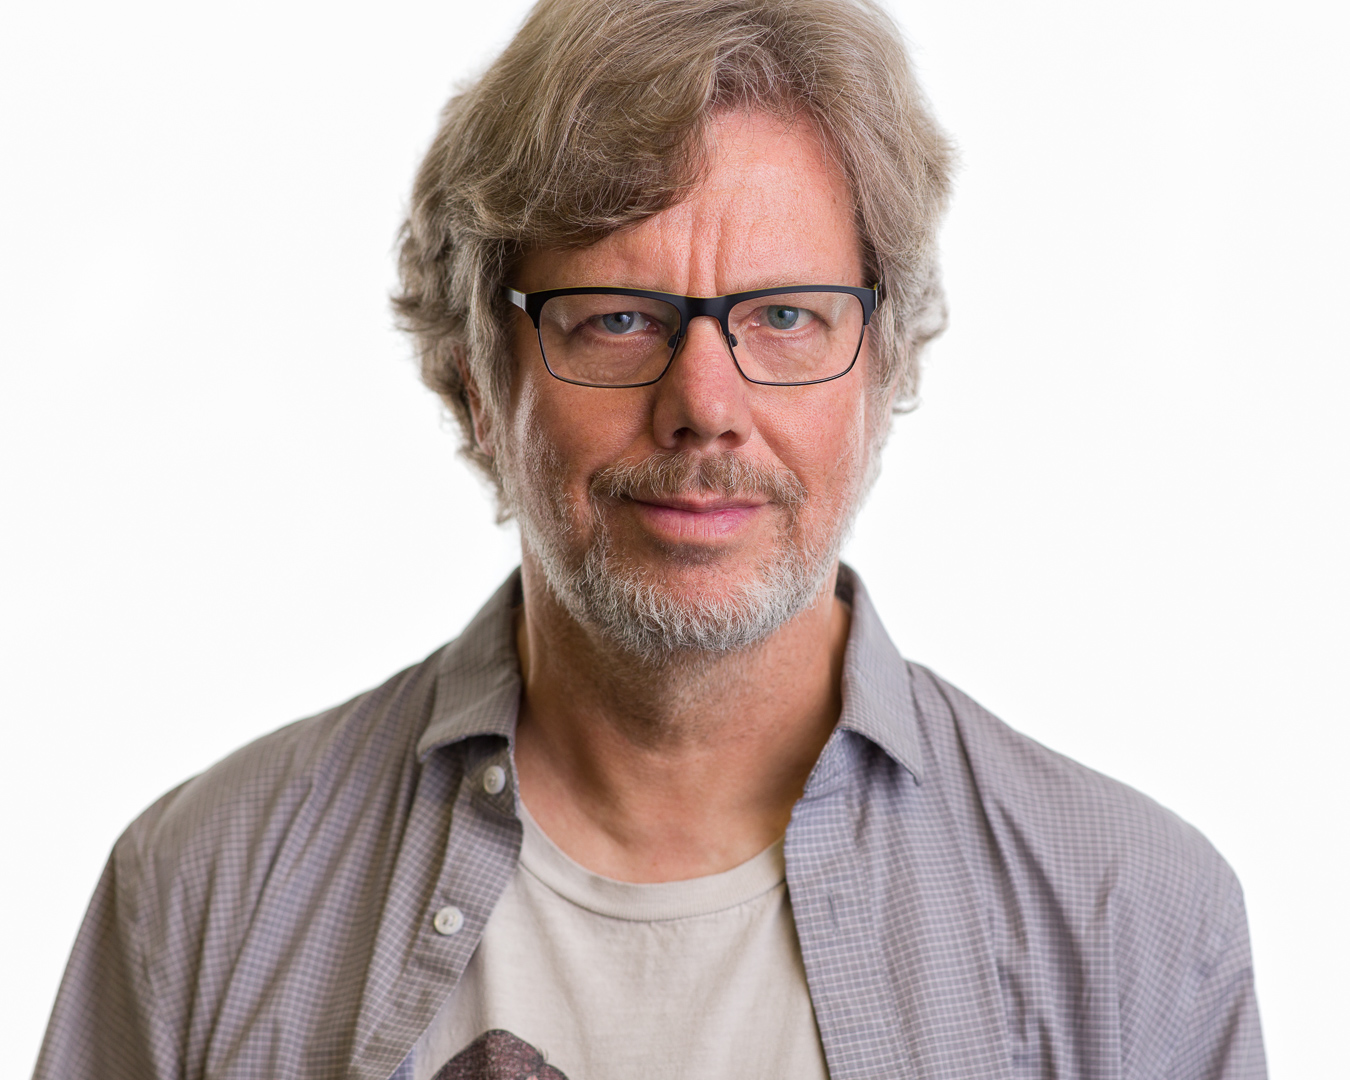
\includegraphics[width=\linewidth]{./Images/Chapter10/graphX-01-van-rossum-2019.jpg}}%
{\href{https://creativecommons.org/licenses/by-nc-nd/4.0/}{\ccbyncndeu\ 4.0} Michael Cavotta}%
Cela peut paraître étonnant, mais \textsc{Python} est relativement ancien, dont la première version publiée remonte à février 1991. Le langage est entré en version 1.0 en janvier 1994 puis en version 2.0 en octobre 2000. À partir de cette date, son essort n'a fait que de s'amplifier.

Inutile de dire qu'à ces débuts le langage ne ressemblait pas exactement à ce qu'on peut utiliser aujourd'hui mais, si le gage de l'ancienneté est synonyme de qualité, \textsc{Python} en bénéficie en ayant pas mal d'heures de vol derrière lui...

Une importante rupture est apparue entre la version\,2 et la version\,3 (décembre 2008). Tout le monde s'accorde à dire que ce fut relativement douloureux, mais nécessaire compte-tenu de, principalement, la manière dont étaient gérées les chaînes de caractères et les encodages. Ces questions seront abordées dans le cours.
Depuis la version 3, évidemment, les choses sont redevenues totalement compatibles. 

Ainsi, le langage a une histoire conséquente, qui n'a connu qu'une seule rupture de compatibilité en quelques trente ans, ce qui, par parallèle à d'autres langages, est tout à fait raisonnable.

Cette évocation permet de mentionner une qualité indéniable de \textsc{Python} : sa stabilité. En effet, la dernière version 2.7 de Python a été maintenue jusqu'en 2020, alors qu'elle était initialement censée devenir obsolète en 2010, lors de la sortie de la version 3.

À l'instar de tous les langages « \textit{mainstream} », \textsc{Python} tient à cœur de rester compatible pendant une très longue durée. 

C'est l'occasion d'aussi noter la pérennité de la bibliothèque standard. Cette bibliothèque --- \textit{library} en anglais --- comporte l'ensemble des utilitaires qui sont empaquetés avec \textsc{Python}. Cela fait partie du langage au sens où cela s'avère intégré à l'installation du langage, mais surtout, que la maintenance est concomitante à celle du langage. En utilisant un morceau de la bibliothèque standard, chacun est assuré de pouvoir l'utiliser dans la durée.

\overparagraph{Portabilité et performances}

\sidegraphic{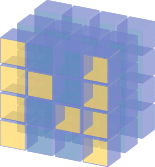
\includegraphics[width=0.75\linewidth]{./Images/Chapter10/numpy-logo.png}}%
Un atout supplémentaire de \textsc{Python} est sa \textit{portabilité}. Autrement dit, un même code va pouvoir fonctionner indifféremment sur une plateforme \textsc{Windows}, \textsc{MacOS} ou \textsc{Linux}. Il s'érige même comme fondation logicielle de certains matériels comme le \textsc{Raspberry Pi}.

\textsc{Python} est un langage multi-facettes qui dispose d'une énorme base de données de code%
\sidenote{%
Calcul scientifique :\setlength{\listindentFB}{4pt}
\begin{itemize}
\jazzitem
	\item \textsc{NumPy}, \textsc{Matplotlib}, \textsc{Scipy}, \textsc{Sympy}.
\end{itemize}
Traitement de données :
\begin{itemize}\jazzitem
	\item \textsc{Pandas}, \textsc{Scikit-Learn}.
\end{itemize}
Internet/Web :
\begin{itemize}\jazzitem
	\item \textsc{Django}, \textit{notebooks} \textsc{Jupyter}.
\end{itemize}
} existant. Au-delà des grands domaines déjà signalés, il est par exemple possible d'écrire un site Web (cf. \href{https://www.djangoproject.com/}{Django}) ou, si besoin se fait sentir, de causer à sa porte de garage ; certainement quelque chose est écrit quelque part pour le faire.

\sidegraphic{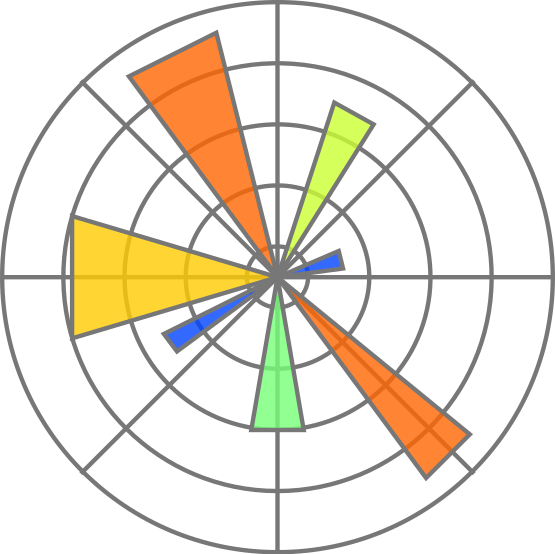
\includegraphics[width=0.75\linewidth]{./Images/Chapter10/matplotlib-logo.png}}%
Une critique assez fréquemment formulée à propos de \textsc{Python} est relative à ses performances. En fait, la plupart du temps, les problèmes qui ont besoin de grosses quantités de cycles\sidenote{Cette critique peut se généraliser à tous les langages interprétés --- même commerciaux comme \textsc{Matlab} --- lorsque, par exemple, il s'agit de réaliser de nombreu\-ses boucles, comme en simulation numérique. Cet inconvénient reçoit le même traitement : en coulisses il est fait appel à des codes compilés pour obtenir des performances comparables avec \textsc{Python}.} ont été réglés en emballant --- \textit{wrapping} en anglais --- du code compilé, typiquement écrit en \textsc{C/C++}, avec une interface \textsc{Python}. Cela s'avère par exemple le cas avec la bibliothèque \textsc{NumPy}, dévolue à la manipulation de tableaux.

\sidegraphic{
\includegraphics[width=0.75\linewidth]{./Images/Chapter10/django-logo.png}}%
En fin de compte, on obtient avec \textsc{Python} un langage où les types de bases sont très puissants, dont les dictionnaires --- abordés plus loin ---, les ensembles ou les tableaux avec \textsc{NumPy}. 
Par ailleurs, la gestion de la mémoire est automatique ; il n'est pas nécessaire de s'attacher à libérer la mémoire. À l'instar de \textsc{Java}, un \textit{garbage collector} --- ramasse-miettes en informatique et littéralement un éboueur --- s'en occupe. 

Tous ces éléments et le fait que \textsc{Python} soit un langage interprété amènent à des développements extrêmement rapides. 

%Enfin, on peut mentionner des outils particuliers comme les \textit{notebooks} \textsc{Jupyter} sur lesquels le cours en ligne se fonde et dont la présentation est à suivre.

\overparagraph{Licence et gouvernance}

%Calqué sur le modèle de la \textit{Free Sofware Foundation}, 

Les droits sont détenus par la \textit{\textsc{Python} Software Foundation}, organisation à but non lucratif. La licence de \textsc{Python} est très permissive, plutôt à rattacher aux licences BSD. Il possible de faire à peu près tout ce que l'on veut, y compris à des fins commerciales.

En terme d'évolutions, parce qu'il y a encore des évolutions aujourd'hui --- comme la programmation asynchrone évoquée dans le cours ---, \textsc{Python} est un langage très vivant. 

La manière de procéder se fonde sur un débat de nature démocratique autour des différentes propositions formulées, puis la décision revient \textit{in fine} au créateur du langage, Guido \textsc{van Rossum} qui, jusqu'en 2018 s'est autoproclamé « dictateur bienveillant à vie » --- \textit{BDFL Benevolent Dictator For Life} --- (comme Linus \textsc{Torwalds} pour le noyau \textsc{Linux}, Larry \textsc{Wall} pour \textsc{Perl} ou Mark \textsc{Shuttleworth} pour \textsc{Ubuntu}). C'est certainement pour cette raison que la cohérence du langage a pu être préservée pendant une durée aussi longue.

Depuis l'été 2018, cette organisation est modifiée avec le retrait partiel de Guido\sidenote{Né en 1956, \textsc{van Rossum} passe progressivement le flambeau et anticipe une retraite bien méritée...} \textsc{van Rossum}. La nouvelle gouvernance s'articule\sidenote{Le \textit{Steering Council} est défini dans la PEP-8016 --- \textit{Python Enhancement Proposal} ---, dont les membres élus sont : Brett Cannon, Nick Coghlan, \href{https://gvanrossum.github.io/}{Guido \textsc{van Rossum}}, \href{https://barry.warsaw.us/}{Barry \textsc{Warsaw}} et \href{https://www.willingconsulting.com/about/}{Carol \textsc{Willing}}.} autour d'un «~\textit{Steering Council} » à traduire en « Conseil de pilotage ».

%\vfill\pagebreak

\begin{gofurther}
\texttitle{Zen de Python}
\begin{itemize}\jazzitem
	\item Le « Zen de Python » résume la philosophie du langage, ce document est disponible en important le module \texttt{this}.
\end{itemize}
\texttitle{Documentation}
\begin{itemize}\jazzitem
	\item Article \href{https://fr.wikipedia.org/wiki/Python_\%28langage\%29}{\textsc{Wikipedia} sur \textsc{Python}}.
	\item Page en \href{https://wiki.python.org/moin/FrenchLanguage}{français} du wiki \textsc{Python}.
	\item Documentation originale de \textsc{Python} v.3 en anglais. C'est un très bon point d'entrée lorsqu'on cherche un sujet particulier, mais (beaucoup) trop abondant pour être lu d'un seul trait. Pour chercher de la documentation sur un module particulier, le plus simple est encore d'utiliser un moteur de recherche qui redirigera, dans la grande majorité des cas, vers la page qui va bien de la documentation de \textsc{Python}.
À titre d'exercice, obtenir la documentation du module \texttt{pathlib} en saisissant les mots-clés « \texttt{python module pathlib} ».
	\item \href{https://docs.python.org/fr/3/}{Traduction française} de la documentation officielle.
\end{itemize}
%\textsc{\lightbf{Survol historique}}
\texttitle{Survol historique}
\begin{itemize}\jazzitem
	\item Foire aux questions (FAQ) officielle de \textsc{Python} (en anglais) sur \href{https://docs.python.org/3/faq/design.html}{les choix de conception et l'historique du langage}.
	\item Article \textsc{Wikipédia} (en anglais) sur l'\href{https://en.wikipedia.org/wiki/History_of_Python}{historique du langage}.
	\item Article \textsc{Wikipédia} (en anglais) sur \href{https://en.wikipedia.org/wiki/Python_syntax_and_semantics}{la syntaxe et la sémantique de Python}.
\end{itemize}
\texttitle{Licence et droits}
\begin{itemize}\jazzitem
	\item \href{https://docs.python.org/3/license.html}{Licence d'exploitation}.
	\item Présentation de la \href{https://www.python.org/psf/}{\textit{\textsc{Python} Software Foundation}}.
\end{itemize}
\texttitle{Développement et gouvernance}
\begin{itemize}\jazzitem
	\item Choix et discussions des évolutions au moyen des PEP, soit \href{https://en.wikipedia.org/wiki/Python_(programming_language)#Development}{\textit{\textsc{Python} Enhancement Proposals}}.
	\item Description du cycle de vie des PEP :\\ \url{https://legacy.python.org/dev/peps/pep-0001/}.
	\item Préconisations du style de présentation (style guide) :\\ \url{https://legacy.python.org/dev/peps/pep-0008/}.
	\item Index de l'ensemble des PEP :\\ \url{https://legacy.python.org/dev/peps/}.
\end{itemize}
\end{gofurther}


\begin{marginvideo}
	[\label{vid:X.3}Environnements de développement : IDLE et interpréteur \textsc{Python}.]%
	\vspace*{-6cm}%
	%\href{./Videos/Chapter09/vidIX-03-idle-HD.mp4}%
	%	{
\includegraphics[width=\marginparwidth]{./Images/Pictograms/film-strip-dark-electric-blue.png}}
	\movie[width=\marginparwidth,showcontrols]%
		{
\includegraphics[width=\marginparwidth]{./Images/Pictograms/film-strip-dark-electric-blue.png}}%
		{./Videos/Chapter10/vidX-03-idle-HD.mp4}%
	\launchvideo{./Videos/Chapter10/vidX-03-idle-HD.mp4}
\end{marginvideo}


%----------
\subsection[Outils de développement]{Outils de développement}
\label{sec:X.1.2}

\caution[t]<firstcolor>{%
L'installation de \textsc{Python} et de ses outils principaux de développement est détaillée en \cref{app:X} \qnameref{app:X}. Les procédures sont exposées en fonction du système d'exploitation.\\
Dans ce document, la position prise est de n'employer que des logiciels libres ou \textit{Open Source}. Par conséquent, l'ensemble des exemples correspond à un environnement de travail fondé sur une base \textsc{Debian}/\textsc{Ubuntu}, en l'occurrence la distribution \textsc{Ubuntu MATE} 20.04 LTS. Sa relative légèreté permet d'envisager l'installer sur des matériels anciens ou des \href{https://ubuntu-mate.org/download/}{\textsc{Raspberry Pi}} (non testé à ce jour).}%
{Installation de \textsc{Python}}%
Une fois l'installation du langage réalisée, il existe essentiellement deux familles d'outils pour communiquer avec \textsc{Python}, soit directement au moyen d'un interpréteur en ligne de commande ou \textit{via} un environnement intégré de développement --- IDE en anglais pour \textit{Integrated Development Environment}.

%\vspace*{-0.5pt}
\subsubsection[Interpréteur \textsc{Python}]{Interpréteur \textsc{Python}}
\label{subsub:X.1.2.1}

L'interpréteur \textsc{Python} est assimilable à un moteur qui fait tourner les programmes. En contexte standard, il n'y a besoin de rien d'autre.

Pour accéder à l'interpréteur Python, il faut d'abord lancer un terminal --- « \textit{shell} » en anglais pour « coque/coquille ». Le terminal est dévolu aux opérations en ligne de commande, à savoir non graphiques, sans IHM (cf. \cref{chap:I}, \qnameref{chap:I}).

Faire appel à un terminal est assez naturel aux utilisateurs de systèmes de type \textsc{Unix} --- par exemple, saisir \keys{Ctrl+Alt+T} sous \textsc{Linux} \textsc{Debian}/\textsc{Ubuntu}. Sous \textsc{Windows}, l'accès au terminal se réalise au moyen de la commande \texttt{cmd}.

Il ne faut pas confondre le terminal, dans lequel des commandes système ou des programmes écrits en langage de \textit{script} « \textit{shell} » --- typiquement en \textit{Bash} pour \textit{Bourne-Again Shell}\sidenote{\textit{Bash} tient son nom du créateur initial de l'interpréteur de commande \textsc{Unix} «\,\texttt{sh}\,» pour \textit{shell}, Stephen \textsc{Bourne}. Sa programmation est à l'origine l'œuvre de Brian \textsc{Fox} dans le cadre du projet GNU (1989). Cette implémentation est désormais celle par défaut des systèmes \textsc{Linux} et \textsc{MacOSX}.} --- peuvent être lancées, avec l'interpréteur \textsc{Python}, même si ce dernier va occuper la même fenêtre de terminal.

Ainsi, à l'invite de commande du terminal, il faut saisir la commande « \texttt{python} » pour lancer l'interpréteur \textsc{Python}. Au préalable, on peut se placer dans un répertoire de travail\sidenote{Remplacer le mot « \texttt{user} » par le nom du compte utilisateur courant.} dévolu aux programmes \textsc{Python}, mettons : \directory{home/user/programming}. 

Sur certains systèmes\sidenote{C'est cas d'\textsc{Ubuntu} 20.4 LTS dont la version 3.8 est installée par défaut, mais où l'appel à \textsc{Python} se réalise toujours par la commande «~\texttt{python3}~».} où coexistent les deux versions 2.7 et 3.x, l'appel à \textsc{Python} en version 3 se fait par la commande « \texttt{python3} ». Ce n'est pas commode, car il faut continuellement se souvenir de quelle version on a besoin, au cas où on aurait velléité d'intervenir sur d'anciens programmes. Cette situation n'a pas lieu d'être ici. Une première chose à faire est donc alors de créer un \textit{alias} de commande dans un des fichiers cachés « \texttt{.bashrc} » ou « \texttt{.bash\_aliases} » de la racine personnelle (cf. procédure : \url{https://doc.ubuntu-fr.org/alias}).


% Just a test
%\setuser{shuser=root, shhost=host, shcolor=white}
%\begin{ubuntu}
%whoami `\startshell`
%root `\setuser{root, shdirectory=/usr}` 
%id `\startshell` 
%uid=0(root) gid=0(root) groups=0(root)`\setuser{root, shdirectory=/usr/bin}`
%hostname `\startshell`
%ubuntu`\setuser{root}`
%ssh bob@remotehost`\startshell`
%bob@remotehost's`\ `password:
%Linux remotehost 2.6.32-5-686 #1 SMP Sun Sep 23 09:49:36 UTC 2012 i686
%You have mail.
%Last login: Wed Oct 16 01:12:35 2012 from localhost
%`\setuser{user}`
%whoami`\startshell`
%bob`\setuser{user}`
%_
%\end{ubuntu}

%\setuser{shuser=user, shhost=host, shcolor=shellusercolor, shprompt char=\$}

\begin{fullwidth}
\setuser{user}
\begin{ubuntu}
sudo ln -s /bin/python3 /bin/python §\startconsole§
[sudo] Mot de passe :
§\setuser{user}§
mkdir programming
cd programming §\setuser{user, shdirectory=/programming}§
python §\startconsole§
Python 3.8.2 (default, Apr 27 2020, 15:53:34) 
[GCC 9.3.0] on linux
Type "help", "copyright", "credits" or "license" for more information.
>>> 20§\shmult§30
600
>>> a=10
>>> print(a)
10
>>> def polynome(x):
...     return 2§\shmult§x§\shmult§§\shmult§2 + 4§\shmult§x + 10
... 
>>> polynome(10)
250
>>> import math
>>> dir(math)
['__doc__', '__loader__', '__name__', '__package__', '__spec__', 'acos', 'acosh', 'asin', 'asinh', 'atan', 'atan2', 'atanh', 'ceil', 'comb', 'copysign', 'cos', 'cosh', 'degrees', 'dist', 'e', 'erf', 'erfc', 'exp', 'expm1', 'fabs', 'factorial', 'floor', 'fmod', 'frexp', 'fsum', 'gamma', 'gcd', 'hypot', 'inf', 'isclose', 'isfinite', 'isinf', 'isnan', 'isqrt', 'ldexp', 'lgamma', 'log', 'log10', 'log1p', 'log2', 'modf', 'nan', 'perm', 'pi', 'pow', 'prod', 'radians', 'remainder', 'sin', 'sinh', 'sqrt', 'tan', 'tanh', 'tau', 'trunc']
>>> help(math.ceil)
Help on built-in function ceil in module math:

ceil(x, /)
    Return the ceiling of x as an Integral.
    
    This is the smallest integer >= x.
(END)

>>> exit() §\setuser{user, shdirectory=/programming}§
python factorielle.py §\startconsole§
3628800 §\setuser{user, shdirectory=/programming}§
\end{ubuntu}
\end{fullwidth}

Néanmoins, si un \textit{alias} s'avère pratique pour l'utilisateur, il ne suffit pas au niveau du système. En effet, si un programme souhaite invoquer \textsc{Python} au moyen de la commande « \texttt{python} », il ne la trouvera pas. La solution est alors de créer un lien symbolique --- en quelque sorte un genre d'\textit{alias} système --- entre les commandes « \texttt{python} » et « \texttt{python3}~» dans le répertoire \directory{/bin} où se trouve l'ensemble des exécutables du système. Si d'aventure cela ne suffisait pas à l'avenir, penser à réitérer la démarche dans le répertoire \directory{/usr/bin}. Les étapes à suivre sont synthétisées dans la simulation\sidenote{Dans la simulation de terminal :
\begin{sideitemize}
  \item le compte utilisateur est « \texttt{user} » ;
  \item la machine hôte est « \texttt{host} ».
\end{sideitemize}} de terminal ci-dessous.

La fenêtre de terminal fait désormais place à l'interpréteur \textsc{Python}. Au passage, on peut remarquer que la version qui est employée est bien en version 3.x et que l'interpréteur \textsc{Python} est bien actif par la présence de son invite de commande spécifique formée de trois chevrons pointant vers la droite. On sort de l'interpréteur pour retourner au \textit{shell} au moyen des commandes « \texttt{quit()} », « \texttt{exit()} » ou en saisissant les touches \keys{Ctrl+D}.

À partir de là, l'interpréteur \textsc{Python} peut s'utiliser, soit comme une grosse calculette, soit pour définir des variables, leur assigner des valeurs et les afficher ou, bien entendu, pour établir des fonctions à la volée en respectant les conventions d'indentation de \textsc{Python}.

% FAUX bien français cf. CNRTL d'échancrure de \textsc{Python} --- \textit{indentation} en anglais, terminologie franglaise tellement usitée en informatique que personne n'en connaît son vocable en français... 

Il est également possible d'importer des bibliothèques externes (cf. l'outil de gestion « \texttt{pip} ») ou, dans le jargon \textsc{Python} des modules avec la commande « \texttt{import <nom-module>} », d'en lister les fonctions disponibles avec « \texttt{dir(<nom-module>)} » et d'obtenir de l'aide sur une fonction par « \texttt{help(<nom-fonction>)} » (sortie avec la touche « \keys{Q} »).

Employer directement l'interpréteur \textsc{Python} est rapidement fastidieux, aussi, on préfère avantageusement construire les développements dans des fichiers séparés --- d'où la création préalable d'un répertoire idoine ---, puis les charger directement depuis le terminal. 

À cet effet et pour illustration par l'exemple, au sein dudit répertoire dédié \directory{/home/user/programming}, on définit un programme dans le fichier\sidenote{Sous \textsc{Ubuntu}, l'éditeur installé par défaut est \texttt{gedit}. Pour le bureau \textsc{MATE}, c'est un \textit{fork} de \texttt{gedit} nommé \texttt{pluma}. Bref, peu importe, faire le choix d'un éditeur de prédilection : \texttt{geany}, \texttt{emacs}, \texttt{vim}, etc.} « \texttt{factorielle.py} » comportant le code ci-dessous. Il est ensuite extrêmement simple d'y faire appel avec la commande (voir la simulation de terminal) : «~\texttt{python factorielle.py} ».

%\ref{code:X.4}% REFERENCE DOES NOT WORK WHY?
\begin{code}{python}[\label{code:X.4}Calcul de factorielle : \texttt{factorielle.py}] 
def factorielle(n):
  """Calcul de factorielle"""
  if n<=1:
    return 1
  else:
    return n*factorielle(n-1)

# Commentaire : factorielle(10) en sortie
print(factorielle(10))
\end{code}

Dans ce cours,%
\caution[t]<firstcolor>{%
Après l'installation de \textsc{IPython} (voir détails en \cref{app:X} \qnameref{app:X}), la même création de lien symbolique est à conduire pour s'assurer de la version correcte du programme. Ainsi, depuis un terminal, il faut saisir :
%\begin{sideitemize}
\texttt{sudo ln −s /bin/ipython3 /bin/ipython}
%\end{sideitemize}
}%
{Agrément pour \textsc{IPython}}
une version améliorée de l'interpréteur \textsc{Python} standard est utilisée, à savoir \textsc{IPython} (à installer en tant que tel).

À l'usage, cet interpréteur bénéficie de fonctionnalités voisines mais plus agréables à manipuler. Il en est ainsi de l'aide en ligne générale, accessible par un point d'interrogation. 

De plus, la complétion (touche \keys{Tab}) est bien plus efficace et pratique, de même que l'indentation qui, cette fois, est automatique et correctement agencée. Par ailleurs, la coloration syntaxique est appliquée par défaut, ce qui facilite rétrospectivement la lecture des instructions \textsc{Python} saisies à la volée.

À titre d'illustration du propos, on peut d'abord importer comme précédemment le module mathématique : « \texttt{import math} ». Avec la complétion, il suffit de saisir le nom du module « \texttt{math.} » et au moyen de la touche \keys{Tab} obtenir la liste des fonctions disponibles. Mais surtout, chose nouvelle, en saisissant de nouveau la touche \keys{Tab}, on peut naviguer sur les fonctions proposées pour s'attacher à l'une d'entre-elles puis, en rajoutant un point d'interrogation, avoir l'aide en ligne qui lui est associée.

En ce qui concerne la coloration syntaxique de \textsc{IPython}, une nouvelle fonction « \texttt{fibonacci} » est définie comme exemple concret d'utilisation (voir simulation de console ci-après). On y constate la notification des mots-clefs du langage.

\vspace*{4pt}

\begin{fullwidth}
\begin{ipythonminted}
§\ipythonuserprompt{user}{host}{~/programming}{\$}\textcolor{white}{ipython}§
§\ipythontext{Python 3.8.2 (default, Apr 27 2020, 15:53:34)}§
§\ipythontext{Type `copyright`, `credits` or `license` for more information}§
§\ipythontext{IPython 7.13.0 -- An enhanced Interactive Python. Type `?` for help.}§

§\ipythonpromptin{1}§ def fibonacci(n):
§\ipythonpromptdots§ return 1 if n <= 1 else fibonacci(n-1) + fibonacci(n-2)
§\ipythonpromptdots§

§\ipythonpromptin{2}§ fibonacci(10)
§\ipythonpromptout{2}§ §\ipythontext{89}§

§\ipythonpromptin{3}§ import math

§\ipythonpromptin{4}§ math.
      §\ipythonmathfunctions§

§\ipythonpromptin{4}§ math.ceil?
§\textcolor{ipythonpromptoutcolor}{Signature:}§ math.ceil(x, /)
§\textcolor{ipythonpromptoutcolor}{Docstring:}§
§\ipythontext{Return the ceiling of x as an Integral.}§

§\ipythontext{This is the smallest integer >= x.}§
§\textcolor{ipythonpromptoutcolor}{Type:}§      builtin_function_or_method

§\ipythonpromptin{5}§ math.ceil(9.5)
§\ipythonpromptout{5}§ §\ipythontext{10}§
\end{ipythonminted}
\end{fullwidth}

\vspace*{6pt}

\subsubsection[IDLE]{\textit{Integrated DeveLopment Environment} --- IDLE}
\label{subsub:X.1.2.2}

Comme bon nombre d'autres langages informatiques, \textsc{Python} dispose d'outils de développement dédiés --- \textit{Integrated Development Environment} ou Environnement de développement intégré (EDI) en français --- facilitant la tâche des programmeurs. Toutes les fonctionnalités nécessaires au développement d'une application sont regroupées au sein d'une même interface de travail. 

Pour ce qui concerne \textsc{Python} et au-delà des EDI généralistes comme \textsc{Eclipse/PyDev} ou les éditeurs multi-facettes comme \textsc{Emacs}, on peut citer les plus connus : \textsc{PyCharm} (licence propriétaire ou communautaire \textsc{Apache}), \textsc{Spyder}\sidenote{\textsc{Spyder} est intéressant à plus d'un titre. Conçu par et pour la communauté \textsc{Python}\linebreak scientifique, ses fonctionnalités le positionne comme une alternative libre à \textsc{Matlab} : interactivité, analyse et visualisation\linebreak de données (\textsc{Matplotlib}), etc. Il peut être étendu par un système de greffons (plug-ins) et, construit sur la bibliothèque graphique \textsc{PyQt}, incorporé dans d'autres programmes comme une de ses extensions.} (sous licence libre MIT, donc sans \textit{copyleft}) et, bien entendu, faisant partie de la distribution\sidenote{Pour \textsc{Linux}, IDLE est disponible comme paquet indépendant pour avoir le choix d'installation d'un EDI de prédilection.} standard, IDLE.

Selon son auteur, Guido \textsc{van Rossum}, l'acronyme officiel de IDLE signifie \textit{Integrated DeveLopment Environment}. Selon d'autres sources, on trouve également l'appellation de : \textit{Integrated Development and Learning Environment}.

IDLE se présente sous la forme d'un \textit{shell} interactif \textsc{Python} (là aussi avec une invite de commande de trois chevrons) qui, nativement, dispose de la coloration syntaxique du code, du surlignage des messages d'erreur, de l'indentation et de l'autocomplétion automatiques des instructions, sans compter d'autres attributs de recherche et de débogage.

Comme pour toute application, pour l'exploiter, il faut la lancer ; quel que soit le système d'exploitation, IDLE est accessible quelque part à partir des menus\sidenote{Pour \textsc{Linux}, installer au préalable le paquet « \texttt{idle} » ou « \texttt{idle3} » avec le gestionnaire de logiciels ou au moyen de la ligne de commande.} du bureau. L'interface obtenue est identique à celle de l'interpréteur \textsc{Python} rencontré précédemment (voir \cref{fig:X.1}).

On peut alors reprendre toutes les opérations effectuées avec l'interpréteur \textsc{Python} (voir \cref{subsub:X.1.2.1}) : de l'utilisation comme calculette à la définition d'instructions et de fonctions à la volée, en passant par la levée d'exception d'erreur et l'aide en ligne. La différence essentielle est que pour saisir une fonction ou un code plus élaboré dans un fichier séparé, il n'y a pas nécessité de sortir de l'environnement mais il suffit simplement d'appeler l'éditeur de texte associé à IDLE : \menu{File>New File}. Une nouvelle fenêtre s'ouvre dans laquelle le code est à entrer.

\begin{jazzfigure*}
\centering
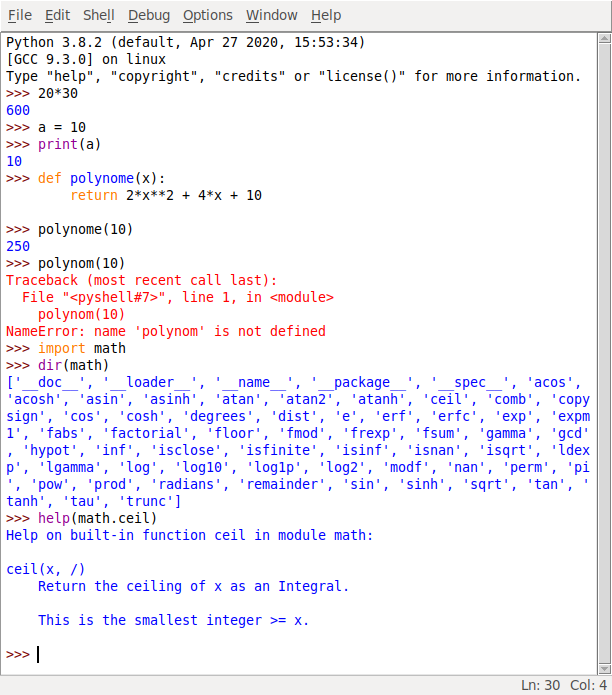
\includegraphics[scale=0.475]{./Images/Chapter10/figX-01a-idleconsole.png}%
\hfill%
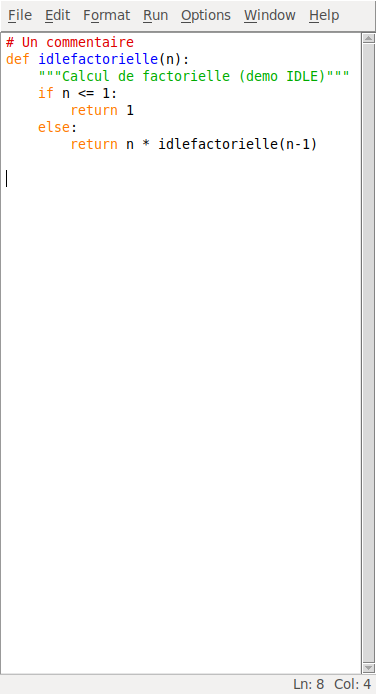
\includegraphics[scale=0.475]{./Images/Chapter10/figX-01b-idleeditor.png}%
\captionsetup{type=figure}%
\caption{\label{fig:X.1}IDLE : console et éditeur de fichier \textsc{Python}.}
\end{jazzfigure*}

Une fois sauvegardé le fichier nouvellement créé en accédant à \menu{File>Save}, ici enregistré sous « \texttt{idlefactorielle.py} », là encore, il n'y a pas besoin de sortir de l'environnement pour exécuter le fichier ; il faut taper la touche de raccourci \keys{F5} ou bien suivre le menu \menu{Run>Run Module}. 

La console de l'interpréteur se réinitialise --- toutes les instructions et variables précédemment introduites sont effacées --- et charge le module. Ce dernier est dès lors fonctionnel et peut s'utiliser par exemple en évaluant \texttt{idlefactorielle(10)}, fonction du module chargé.

Cette boucle interactive est le principe de travail avec IDLE et tout autre environnement de développement intégré : on introduit le nouveau code dans un fichier, on valide en sauvegardant puis on passe la main à l’interpréteur pour vérifier le résultat ; et ainsi de suite...

D'un EDI à l'autre et au-delà de leurs fonctionnalités propres --- visualisation de données, développement Web avec \textsc{Django}, etc. ---, seule l'interface de présentation change. Juste à titre de comparaison, la \cref{fig:X.2} montre l'interface utilisateur de \textsc{Spyder}, qui intègre dans le même espace de travail un éditeur de fichier, une console \textsc{IPython} et un volet d'exploration de fichiers ou d'affichage de l'aide en ligne.

\begin{jazzfigure*}
\centering
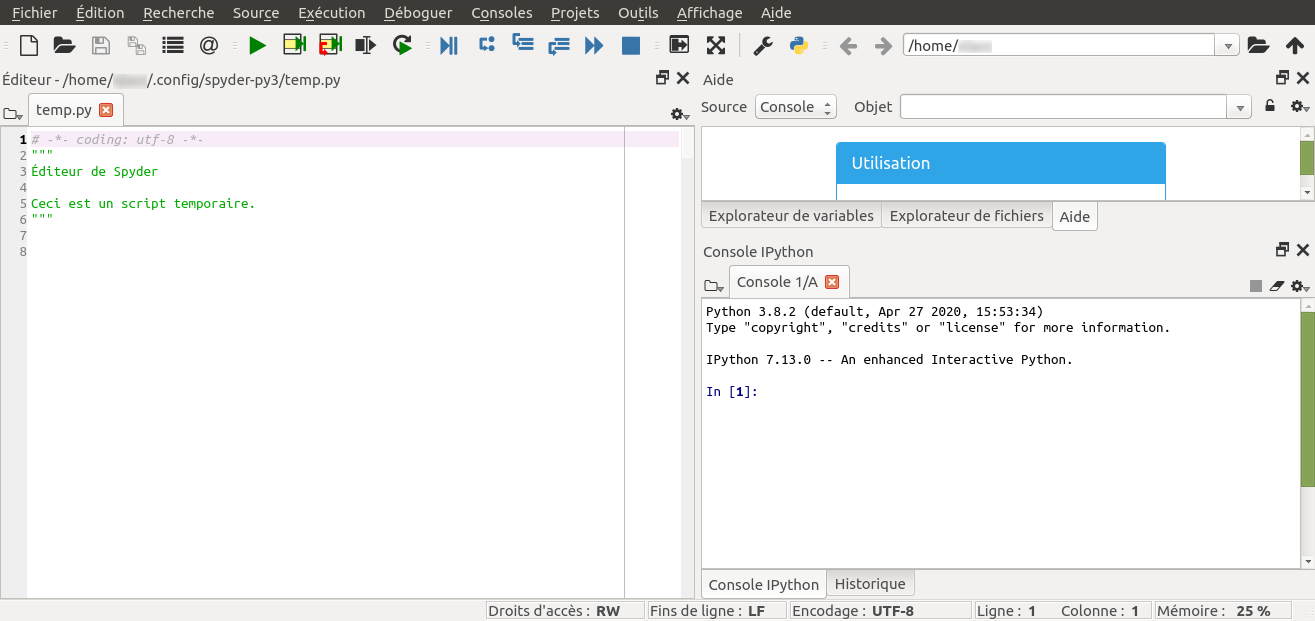
\includegraphics[width=\linewidth]{./Images/Chapter10/figX-02-spyder.png}%
\captionsetup{type=figure}%
\caption{\label{fig:X.2}Interface utilisateur de \textsc{Spyder}.}
\end{jazzfigure*}


%\subsubsection[Exemples d'utilisation]{Exemples d'utilisation}
%\label{subsub:X.1.2.3}

%\subsubsection[Éléments additionnels]{Éléments additionnels}
%\label{subsub:X.1.2.4}


%-----
\subsection[Documentation et code \textsc{Python}]{Documentation et code \textsc{Python}}
\label{sub:X.1.3}

\begin{marginvideo}
	[\label{vid:X.4}\emph{Notebooks} \textsc{Jupyter}.]%
	%\href{./Videos/Chapter09/vidIX-04-notebooks-HD.mp4}%
	%	{
\includegraphics[width=\marginparwidth]{./Images/Pictograms/film-strip-dark-electric-blue.png}}
	\movie[width=\marginparwidth,showcontrols]%
		{
\includegraphics[width=\marginparwidth]{./Images/Pictograms/film-strip-dark-electric-blue.png}}%
		{./Videos/Chapter10/vidX-04-notebooks-HD.mp4}%
	\launchvideo{./Videos/Chapter10/vidX-04-notebooks-HD.mp4}
\end{marginvideo}

Au fur et à mesure des années et, tout particulièrement dans la dé\-cennie 2010--2020, les outils de documentation et d'apprentissage de l'informatique se sont considérablement améliorés. L’essor de l'Internet y a largement contribué, à l'exemple de certains langages de balisage léger permettant la mise en exergue des codes.

Pour les documentations écrites, les outils de composition \TeX\ (1983) puis \LaTeX\ (1994) restent maîtres en la manœuvre, à l'image de ce document. Néanmoins, un minimum d'interactivité est apportée par l'extension \textsc{Python}\TeX\ (depuis 2012), succinctement présentée en \cref{subsub:X.1.3.2}.

En revanche, les \textit{notebooks} \textsc{Jupyter} (2015) apportent une interactivité complète entre présentation de données textuelles --- cours et explications --- et de codes modifiables à volonté --- manipulations et tests. Cela offre un outil pédagogique efficient pour l'apprentissage d'un langage de programmation.

%(nul besoin d'abondance de commentaires au sein des codes).


\subsubsection[« \textit{Notebooks} » \textsc{Jupyter}]{« \textit{Notebooks} » \textsc{Jupyter}}
\label{subsub:X.1.3.1}

\sidegraphic{
\includegraphics[width=0.75\linewidth]{jupyter-logo.png}}%
Que recouvre donc la terminologie de \textit{notebooks} \textsc{Jupyter} ? 

En premier lieu et par contraste avec les outils auparavant présentés, le système de \textit{notebooks} n'a pas besoin d'être installé en local\sidenote{Sauf pour travailler sans connexion Internet ou développer soi-même une documentation sur ce principe.} sur la machine de l'utilisateur ; il est hébergé sur une plateforme distante pour permettre le travail en ligne.

Un \textit{nootebook} est ainsi un mélange de texte et de code. On navigue au sein de ses différentes cellules au moyen de la suite de touches \keys{Maj+Entrée}. Tant que l'on est sur du texte cela importe peu. En revanche, sur une cellule de code, la saisie des touches \keys{Maj+Entrée} active le code contenu et le communique à l'interpréteur qui renvoie le résultat.

De cette manière, on peut lire linéairement le document du début à la fin en évaluant le code au fur et à mesure où, à chaque fois qu'une cellule de code est rencontrée, son label entre crochets est incrémenté d'une unité. Cela représente le degré zéro de l'utilisation d'un \textit{notebook}. On peut également mentionner que l'ensemble du \textit{notebook} est évalué en une seule opération avec \menu{Cell>Run All}.

\caution[t]<secondcolor>{%
Pour le bon fonctionnement des \textit{note\-books}, il faut avoir autorisé le navigateur Web à accepter les cookies en provenance du site \url{https://nbhosting.inria.fr}, qui héberge l'infrastructure du \textsc{Mooc}.}{Attention !}
Comme pour tous les programmes à interface graphique, les \textit{notebooks} disposent de barres de menu et de raccourcis (cf. \cref{fig:X.3}). Il est néanmoins conseillé, par souci d'efficacité, de retenir les quelques raccourcis clavier qui rendre la consultation plus fluide.

Lorsqu'une cellule de code est évaluée, \textsc{Jupyter} ajoute sous la cellule \texttt{In} une cellule \texttt{Out} qui donne le résultat du fragment \textsc{Python} considéré, soit \texttt{600} dans le premier exemple de la \cref{fig:X.4}.

\sidefigure[\label{fig:X.3}Barres de menu et de raccourcis d'un \emph{notebook} \textsc{Jupyter}.]%
{
\includegraphics[width=0.925\marginparwidth]{./Images/Chapter10/figX-04a-nbmenu.png}\\[2pt]
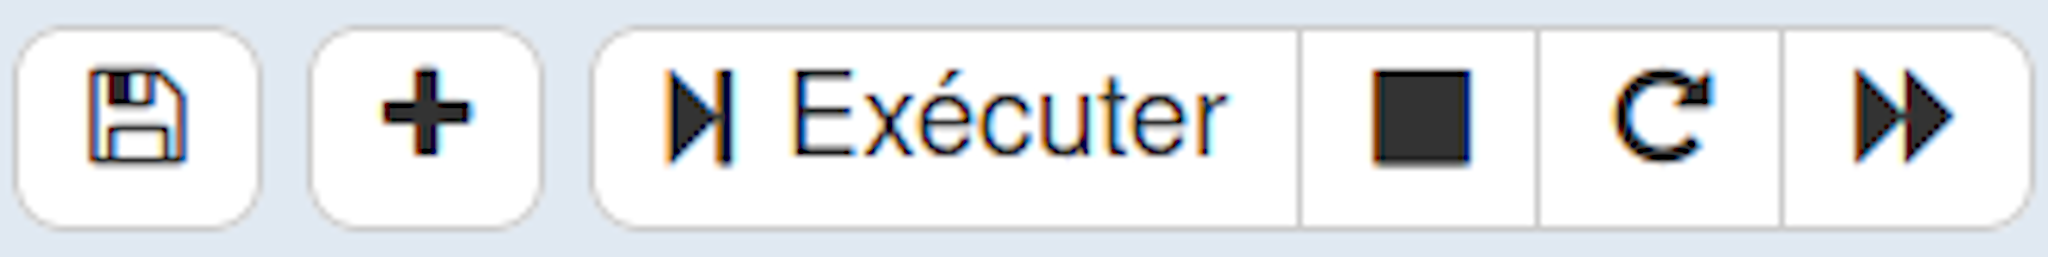
\includegraphics[width=\marginparwidth]{./Images/Chapter10/figX-04b-nbshortcuts.png}}%
En seconde instance, on peut revenir sur une cellule de code pour en modifier les paramètres et de nouveau en tapant \keys{Maj+Entrée}, réévaluer le résultat retourné par la cellule.

Ces premières étapes sont reprises par la \cref{fig:X.4} où sont évaluées deux celulles de codes telles que présentées initialement puis après modification par l'utilisateur.

\begin{figure}
\begin{nbjupyterin}{1}
20 * 30
\end{nbjupyterin}
\begin{nbjupyterout}{1}
600
\end{nbjupyterout}
\begin{nbjupyterin}{1}
20 * 40
\end{nbjupyterin}
\begin{nbjupyterout}{1}
800
\end{nbjupyterout}
\begin{nbjupyterin}{2}
# math.sqrt (pour square root) calcule la racine carrée
import math
math.sqrt(2)
\end{nbjupyterin}
\begin{nbjupyterout}{2}
1.4142135623730951
\end{nbjupyterout}
\begin{nbjupyterin}{2}
# math.sqrt (pour square root) calcule la racine carrée
import math
math.sqrt(25)
\end{nbjupyterin}
\begin{nbjupyterout}{2}
5
\end{nbjupyterout}
\caption{\label{fig:X.4}Évaluation et modification de cellules de code \emph{notebook} \textsc{Jupyter}.}
\end{figure}

\vspace*{-2pt}

L'intérêt du numéro entre crochets des cellules contenant du code est de suivre l'ordre dans lequel celles-ci sont évaluées : on peut tout à fait sauter certaines cellules dans le fil de lecture pour y revenir ensuite. Toutefois, cela devient rapidement confus et s'avère \emph{fortement déconseillé} car pouvant mener à des résultats inattendus selon la progression pédagogique voulue du \textit{notebook}. 

En effet, les cellules de code peuvent être des fragments d'un même programme \textsc{Python} ; les exécuter dans le désordre produit un ensemble différent, voire incohérent. La \cref{fig:X.5} expose une telle situation.

\begin{figure}
\begin{nbjupyterin}{1}
message = "Faites attention à l'ordre dans lequel vous évaluez les notebooks"
\end{nbjupyterin}
\vspace*{1pt}
\begin{nbjupyterin}{3}
print(message)
----------------------------------------------------------------
NameError                      Traceback (most recent call last)
<ipython-input-3-83cfdf559502> in <module>
----> 1 print(message)

NameError: name 'message' is not defined
\end{nbjupyterin}
\vspace*{1pt}
\begin{nbjupyterin}{2}
# ceci a pour effet d'effacer la variable 'message'
del message
\end{nbjupyterin}
%\vspace*{6pt}
\caption{\label{fig:X.5}Évaluation désordonnée de cellules de code \emph{notebook} \textsc{Jupyter}.}
\vspace{-\baselineskip}
\end{figure}

On peut avoir besoin de réinitialiser le \textit{notebook} après avoir réalisé trop de modifications ou perdu le fil de ce qui a été évalué. Pour ce faire, il faut aller dans le menu du \textit{notebook} pour faire un \menu{Kernel>Restart} ou mieux, \menu{Kernel>Restart \& Clear Output}, autre\-ment dit, non seulement redémarrer le noyau, mais aussi remettre à zéro tous les affichages.

\begin{figure}[th]
\begin{nbjupyterin}{1}
# Il faut exécuter cette cellule pour charger l'exercice
from corrections.w1s3_polynome import exo_polynome
\end{nbjupyterin}
\vspace*{4pt}
\begin{nbjupyterin}{2}
# Une cellule de ce genre est destinée à montrer le résultat attendu
exo_polynome.example()
\end{nbjupyterin}
\begin{nbjupyterout}{2}
Appel          Attendu
polynome(-2)    4
polynome(0)    -4
\end{nbjupyterout}
\begin{nbjupyterin}{\,}
# Le code proposé est à entrer ici
def polynome(x):
    "votre code"
\end{nbjupyterin}
\vspace*{4pt}
\begin{nbjupyterin}{3}
# Le code proposé est à entrer ici (oubli de l'instruction `return')
def polynome(x):
    2*x**2-4
\end{nbjupyterin}
\vspace*{4pt}
\begin{nbjupyterin}{4}
# Une fois exécuté la cellule précédente avec votre code,
# il faut évaluer celle-ci pour vérifier si cela fonctionne
exo_polynome.correction(polynome)
\end{nbjupyterin}
\begin{nbjupyterout}[colback=pynbcodefalsebgcolor]{4}
Appel          Attendu      Obtenu
polynome(-2)     4           None     NO
polynome(0)     -4           None     NO
polynome(2)      4           None     NO
\end{nbjupyterout}
\begin{nbjupyterin}{3}
# Le code proposé est à entrer ici
def polynome(x):
    return 2*x**2-4
\end{nbjupyterin}
\vspace*{4pt}
\begin{nbjupyterin}{4}
# Une fois exécuté la cellule précédente avec votre code,
# il faut évaluer celle-ci pour vérifier si cela fonctionne
exo_polynome.correction(polynome)
\end{nbjupyterin}
\begin{nbjupyterout}[colback=pynbcodetruebgcolor]{4}
Appel          Attendu      Obtenu
polynome(-2)     4             4      OK
polynome(0)     -4            -4      OK
polynome(2)      4             4      OK
\end{nbjupyterout}
\vspace*{2pt}
\caption{\label{fig:X.6}Exercice auto-évalué.}
%\vspace{-\baselineskip}
\end{figure}
%polynome(0)      4             4      OK
%polynome(-10)  196           196      OK

\vspace*{-2pt}

Un point important à connaître est que l'utilisateur \emph{travaille sur une copie de la proposition initiale}. Toutes les modifications qui sont faites par l'utilisateur lui appartiennent et peuvent être sauvegardées. Elles le sont automatiquement, mais si on souhaite disposer d'une progression plus fine, suivre le menu \menu{File>Save} ou \menu{File>Save as...}.

À tout moment, la version initiale du \textit{notebook} peut être rechargée en suivant \menu{File>Reset to Original} ; faire attention au code saisi auparavant, car il va bien entendu être écrasé.

Une autre fonctionnalité intéressante est de pouvoir télécharger le contenu du \textit{notebook} dans de multiples formats et notamment en \textsc{Python} : \menu{File>Download as>Python (.py)}. Pour ce dernier format, les cellules de texte sont préservées sous forme de commentaires \textsc{Python}, seules les cellules de code sont actives.

En contexte de partage d'expérience, comme par exemple en formation à distance, il est encore possible de publier une version HTML statique du fruit du travail d'un étudiant donné : \menu{File>Share Static Version}. Une URL est obtenue afin d'être publiée dans un forum d'aide ou envoyée par courriel. Ainsi, les autres participants accèdent en lecture seule au code. Cette manipulation peut se réaliser plusieurs fois : c'est toujours la dernière version qui est partagée --- l'URL reste la même pour un étudiant et un \textit{notebook} donnés.

% Like \sidefigure/marginfigure bug in the list of... WHY?
\sidetable[\label{tab:X.1}Fonctionnalités d'un \emph{notebook} \textsc{Jupyter}.]{%
%\begin{margintable}
%\caption{\label{tab:X.1}Fonctionnalités d'un \emph{notebook} \textsc{Jupyter}.}%
\begingroup
\footnotesize
\renewcommand*{\arraystretch}{1.6}
\rowcolors{2}{tableLineOne}{tableLineTwo}
\begin{tabularx}{\marginparwidth}{YY}
\rowcolor{secondcolor}
\multicolumn{2}{c}{\Gape[6pt]{\textcolor{white}{\textbf{Commandes et raccourcis}}}} \\
\rowcolor{firstcolor}
\multicolumn{1}{c}{\scshape\titlingfont\textcolor{white}{Action}} 
	& \multicolumn{1}{c}{\scshape\titlingfont\textcolor{white}{Clavier}} \\
Déplacement/ Évaluation & \keys{Maj+Entrée} \\
\rowcolor{firstcolor}
\multicolumn{1}{c}{\scshape\titlingfont\textcolor{white}{Action}} 
	& \multicolumn{1}{c}{\scshape\titlingfont\textcolor{white}{Menu}} \\
Évaluation globale & \menu{Cell>Run All} \\
Réinitialisation & \menu{Kernel>Restart} \\
Réinitialisation et remise à zéro & \menu{Kernel>Restart Clear Out.} \\
Enregistrement & \menu{File>Save} \\
Version originale & \menu{File>Reset to Original} \\
Téléchargement & \menu{File>Download as} \\
Lien partagé (URL/HTML) & \menu{File>Share Stat. Vers.} \\
Insertion cellule & \menu{Insert} \\
\rowcolor{firstcolor}
\multicolumn{1}{c}{\scshape\titlingfont\textcolor{white}{Action}} 
	& \multicolumn{1}{c}{\scshape\titlingfont\textcolor{white}{Raccourci}} \\
Évaluation & \faStepForward \\ %\faPlay\rule[-0.5pt]{1pt}{6.5pt} \\
Insertion après & \faPlus \\
Interruption & \faStop \\ %du noyau
Redémarrage avec confirm. & \faRedo \\ %du noyau
Redémarrage sans confirm. & \faForward \\ %du noyau
\end{tabularx}% "%" est nécessaire pour éviter une alerte "underfull box"
\endgroup
%\end{margintable}
}

Enfin, des cellules supplémentaires peuvent être rajoutées : \menu{Insert>Insert Cell Above} ou \menu{Insert>Insert Cell Below}. Arrivé à la fin d'un document, chaque fois que la dernière cellule est évaluée, cela crée une nouvel\-le cellule. De cette manière, on dispose d'un brouillon pour effectuer des tests personnels concernant les sujets abordés par le \textit{notebook} en cours de consultation.

La \cref{tab:X.1} reprend les différentes actions possibles sur un \textit{notebook} \textsc{Jupyter} avec leur commandes associées.

\paragraph*{Exercices auto-évalués} Le Mooc propose un certain nombre d'exercices à réaliser en autonomie, dont la correction est guidée par les réponses apportées, d'où le terme d'\emph{auto-évalué}.

Au sein d'un \textit{notebook}, un énoncé est formulé. À titre d'exemple, le propos est d'écrire une fonction qui implémente le polynôme $2x^2 - 4$ (cf. \cref{fig:X.6}). La manière de procéder est toujours la même, à savoir évaluer les cellules à l'aide des touches \keys{Maj+Entrée}. 

L'évaluation de la première cellule d'exercice est fondamentale, car c'est elle qui charge son contenu. Les résultats attendus sont ensuite exposés dans la cellule suivante de manière à orienter les sorties du code à produire (voir \cref{fig:X.6}).

La cellule encore suivante est ouverte au sens où elle est le réceptacle du code à proposer pour résoudre le problème énoncé. Une fois remplie, on passe à la cellule subséquente qui fournit la correction de la réponse donnée. 

En cas d'échec, une sortie explicite (fond rouge) est renvoyée entre les attendus et les résultats actuels. En cas de succès, il en est de même, mais la comparaison (fond vert) entre attendus et résultats est bien entendu positive. On peut évaluer ces deux dernières cellules autant de fois qu'il est nécessaire pour atteindre une correction correcte (cf. \cref{fig:X.6} où les deux situations sont illustrées : réponse fausse et résultat correct).


\subsubsection[Extension \LaTeX\ \textsc{Python}\TeX]{Extension \LaTeX\ \textsc{Python}\TeX}
\label{subsub:X.1.3.2}

Les quelques paragraphes à suivre n'ont aucun rapport direct avec le \textsc{Mooc}, ils offrent juste quelques éléments d'information supplémentaire aux personnes qui, maîtrisant correctement \LaTeX, souhaiteraient reprendre ce document ou en rédiger un nouveau.

L'installation et l'emploi des outils de composition \LaTeX\ utilisés pour ce document sont exposées en annexe. Il s'agit uniquement de mentionner une des extensions utilisées, \textsc{Python}\TeX, qui apporte un minimum d'interactivité entre un document \LaTeX\ et des syntaxes ou des programmes \textsc{Python} qui sont à présenter et à expliquer. %\cref{app:X} \qnameref{app:X}

\LaTeX\ est un langage de balisage qui permet la mise en forme de documents de qualité, mais qui, contrairement à par exemple HTML, nécessite une phase de compilation pour passer d'un fichier texte source à un document PDF (pour simplifier). La procédure habituelle est donc de lancer un programme --- en pratique \texttt{pdflatex} ou \texttt{lualatex} --- pour gérer cette conversion : \texttt{pdflatex fichier.tex} pour avoir \texttt{fichier.pdf}.

Dans la conversion vers le format PDF, un certain nombre de fichiers auxiliaires sont également générer pour correctement afficher les références croisées (numéros de figure, table, équation, etc.). Plusieurs compilations sont alors nécessaires pour que soit stabilisé le fichier final en PDF. C'est le prix à payer de la qualité typographique et de la précision en regard d'autres traitements de texte traditionnels.

Dans ce processus, l'extension \textsc{Python}\TeX\ s'insère en tant qu'étape intermédiaire entre le fichier source et le résultat PDF, au même titre que la nécessité de compilations multiples (en pratique deux ou trois). C'est-à-dire que la procédure devient désormais : \texttt{pdflatex fichier} \faCaretRight\space \texttt{pythontex fichier} \faCaretRight\space \texttt{pdflatex fichier} où \texttt{pythontex} est un \textit{script} \textsc{Python} qui s'occupe d'interpréter du code \textsc{Python}, en l'occurence.

Certes, fort bien, mais quelle\sidenote{Au passage, cela montre la polyvalence et la puissance de \textsc{Python} dans de multiples champs d'ap\-plication.} est la plus-value ? L'intérêt est que, moyennant une syntaxe adéquate, il est possible depuis un document \LaTeX\ d'envoyer du code \textsc{Python} pour interprétation et d'en récupérer le résultat pour sa mise en forme au sein d'un document. Tout comme pour les \textit{notebooks}, la bibliothèque d'affichage des codes est \texttt{Pygments}.

À l'évidence, cette solution est moins interactive qu'un \textit{notebook} \textsc{Jupyter}, mais s'avère très performante dans le cadre de la rédaction de manuels ou d'ouvrages de programmation informatique (\textsc{Python} n'est pas le seul langage supporté, cf. documentation \href{https://ctan.org/pkg/pythontex}{CTAN \textsc{Python}\TeX}).


%-----
\subsection[Synthèse et compléments]{Synthèse et compléments}
\label{sub:X.1.4}

Après l'abord des généralités à propos des contextes d'utilisation du langage \textsc{Python}, une petite synthèse est menée et quelques exercices simples sont proposés pour avancer un peu plus.


\subsubsection[Modes d'exécution \textsc{Python}]{Mode d'exécution \textsc{Python}}
\label{subsub:X.1.4.1}

Les différents modes d'exécution d'un programme \textsc{Python} sont résumés en \cref{tab:X.2}. Il s'agit maintenant de les étudier en détail. Pour cela, le comportement d'un tout petit programme va être regardé lorsqu'on l'exécute sous ces différents environnements.

\sidetable[\label{tab:X.2}Modes d'exécution \textsc{Python}.]{%
\begingroup
\renewcommand*{\arraystretch}{1.6}
\rowcolors{2}{tableLineOne}{tableLineTwo}
\begin{tabularx}{\marginparwidth}{lY}
\rowcolor{secondcolor}
\multicolumn{2}{c}{\Gape[6pt]{\textcolor{white}{\textbf{Exécution d'un programme \textsc{Python}}}}} \\
\rowcolor{firstcolor}
\multicolumn{1}{c}{\scshape\titlingfont\textcolor{white}{Quoi ?}} 
	& \multicolumn{1}{c}{\scshape\titlingfont\textcolor{white}{Comment ?}} \\
Fichier entier & \texttt{python <fichier>.py} \\
Ligne à ligne   & IDLE, \texttt{ipython}, \texttt{python} mode interactif \\
Par fragment    & \textit{notebook} \\
\end{tabularx}%
\endgroup
}

Essentiellement, lorsqu'on utilise l'interpréteur en mode interactif --- ou sous IDLE ---, à chaque fois que l'on tape une ligne, le résultat est \emph{calculé} (on dit aussi \emph{évalué}) puis \emph{affiché}.

En revanche, lorsqu'on écrit tout un programme, on ne peut plus imprimer le résultat de toutes les lignes, cela produirait un flot de données beaucoup trop important. Par conséquent, si on ne déclenche pas un affichage explicite avec, par exemple, la fonction \texttt{print}, rien ne se se produit en sortie.

En ce qui concerne le \textit{notebook}, le comportement est un peu hybride entre les deux, en ce sens que seul le \emph{dernier résultat} de la cellule est affiché.

Le programme qui sert ici d'illustration est simplissime.
\begin{listingbox}[after skip=6pt]{python}
10 * 10
20 * 20
30 * 30
\end{listingbox}

Lorsque ces instructions sont soumises à l'interpréteur interactif (ouvrir un terminal, puis appeler \texttt{python}), on obtient :
\vspace*{4pt}
\begin{ubuntu}
python §\startconsole§
Python 3.8.2 (default, Apr 27 2020, 15:53:34) 
[GCC 9.3.0] on linux
Type "help", "copyright", "credits" or "license" for more information.
>>> 10 * 10
100
>>> 20 * 20
400
>>> 30 * 30
900
>>> exit() §\setuser{user}§
§ §
\end{ubuntu}
\vspace*{4pt}

À noter que pour sortir de l'interpréteur, il faut saisir \texttt{exit()} --- ou sous \textsc{Linux} et \textsc{MacOSX} \keys{Ctrl+Entrée}.

Que donne à présent cette même séquence de calculs dans un programme complet ? Pour cela, il faut tout d'abord fabriquer un fichier ayant pour suffixe \texttt{.py}, au moyen par exemple d'un éditeur de fichier, puis exécuter le programme ainsi obtenu. Le résultat doit ressembler à ceci (la fonction \texttt{cat} est une instruction \textsc{Unix} qui permet de concaténer et/ou définir un fichier en ligne de commande) :
\vspace*{4pt}
\begin{ubuntu}
cat > foo.py << EOF §\startconsole§
> 10 * 10
> 20 * 20
> 30 * 30
> EOF §\setuser{user}§
cat foo.py §\startconsole§
10 * 10
20 * 20
30 * 30 §\setuser{user}§
python foo.py
§ §
\end{ubuntu}
\vspace*{4pt}

Tout au moins en apparence, ce programme semble \emph{ne rien faire} !

En réalité, les trois valeurs \texttt{100}, \texttt{400} et \texttt{900} sont bien calculées, mais comme aucune instruction \texttt{print} n'est présente, rien ne s'affiche et le programme se termine sans signe apparent d'avoir fonctionné.

Ce comportement peut paraître un peu déroutant au début, mais comme déjà mentionné c'est tout à fait délibéré. Avec un programme fonctionnel faisant facilement plusieurs milliers de lignes, voire beaucoup plus, il ne serait pas du tout réaliste que chaque ligne produise une impression, comme c'est le cas en mode interactif.

En exécutant cette fois la même série d'instructions dans un \textit{notebook} (par sélection de la cellule, puis saisie de \keys{Maj+Entrée}), on a :
\begin{nbjupyterin}[before skip=4pt, after skip=1pt]{1}
10 * 10
20 * 20
30 * 30
\end{nbjupyterin}
\begin{nbjupyterout}[after skip=2pt]{1}
900
\end{nbjupyterout}

Une seule valeur est obtenue en sortie --- rubrique \texttt{Out[]} ---, en l'occurrence \texttt{900}, qui correspond bien au \emph{résultat de la dernière ligne}.


\paragraph*{Utilisation de l'instruction d'affichage} Ainsi, pour afficher un résultat intermédiaire, on emploie l'instruction \texttt{print}. Son étude est abordée en détail plus loin dans le \textsc{Mooc}, mais en guise d'introduction, disons seulement que c'est une fonction comme les autres en \textsc{Python} v.3.x.

\begin{nbjupyterin}[before skip=4pt, after skip=1pt]{1}
a = 10
b = 20
print (a, b)
\end{nbjupyterin}
\begin{nbjupyterout}[before skip=4pt, after skip=0pt]{1}
10 20
\end{nbjupyterout}

On peut naturellement mélanger des objets de plusieurs types et donc combiner des chaînes de caractères et des nombres pour obtenir un résultat un peu plus lisible. En effet, lorsque le programme devient volumineux, il est important de savoir à quoi correspond une ligne dans le flot de tous les affichages. Aussi on préférera quelque chose comme :

\begin{nbjupyterin}[before skip=4pt, after skip=2pt]{2}
print("a =", a, "et b =", b)
\end{nbjupyterin}
\begin{nbjupyterout}[before skip=1pt]{2}
a = 10 et b = 20
\end{nbjupyterout}

\begin{nbjupyterin}[before skip=4pt, after skip=2pt]{3}
# ou encore, de manière équivalente mais avec un f-string
print(f"a = {a} et b = {b}")
\end{nbjupyterin}
\begin{nbjupyterout}[before skip=1pt, after skip=4pt]{3}
a = 10 et b = 20
\end{nbjupyterout}

Une pratique courante consiste d'ailleurs à utiliser les commentai\-res pour laisser dans le code les instructions \texttt{print} qui correspondent à du débogage (c'est-à-dire qui ont pu être utiles lors de la mise au point et qu'on veut pouvoir réactiver rapidement).

Remarquons enfin que l'affectation à une variable ne retourne aucun résultat.
Autrement dit, en pratique, que si on écrit :

\begin{nbjupyterin}[before skip=4pt, after skip=4pt]{4}
a = 100
\end{nbjupyterin}
\noindent même une fois l'expression évaluée par l'interpréteur, aucune ligne de sortie \texttt{Out[]} n'est ajoutée.

C'est pourquoi, il arrive parfois d'écrire, notamment lorsque l'expression est complexe et pour rendre explicite la valeur qui vient d'être affectée :

\begin{nbjupyterin}[before skip=4pt, after skip=2pt]{5}
a = 100; print(a)
\end{nbjupyterin}
\begin{nbjupyterout}[before skip=1pt, after skip=6pt]{5}
100
\end{nbjupyterout}

Bien noter que cette technique est uniquement pédagogique et n'a absolument aucun autre intérêt dans la pratique ; il n'est \emph{pas recommandé} de l'utiliser en dehors de ce contexte.

\paragraph*{Ligne d'invite \textit{Shebang}} Pour finir sur les modes d'exécution de \textsc{Python}, une fonctionnalité pratique est à connaître, mais uniquement valable pour les systèmes Unix (\textsc{Linux} et \textsc{MacOSX}).

Le lancement d'un programme Python s'effectue depuis le terminal par la commande : \texttt{python mon\_module.py}.
Lorsqu'il s'agit d'un programme que l'on utilise fréquemment, on n'est pas forcément dans le répertoire où se trouve le programme \textsc{Python}. Aussi, on peut alors utiliser un chemin  « absolu », c'est-à-dire à partir de la racine des noms de fichiers, comme : \texttt{python /le/chemin/de/mon\_module.py}. Cependant, c'est assez malcommode et cela devient vite pénible à la longue.

Sur \textsc{Linux} et \textsc{MacOSX}, il existe une astuce utile pour simplifier cela. En prenant par exemple le programme \texttt{fibonacci.py} de l'exercice d'application à suivre (cf. \cref{subsub:X.1.4.2}), on l'édite avec un éditeur de texte pour lui rajouter une \emph{toute première ligne} qui commence par un caractère de commentaire « \texttt{\#} », seul caractère qui, du à sa position dans le fichier, n'a pas la signification de début de commentaire mais, par la présence d'un point d'exclamation immédiatement après le caractère dièse rend active la suite de la ligne comme chemin d'accès à l'interpréteur \textsc{Python} (voir ci-dessous). Ceci s'appelle un \href{https://en.wikipedia.org/wiki/Shebang_%28Unix%29}{\texttt{shebang}} dans le jargon \textsc{Unix}, rendu possible grâce aux variables d’environnement de ce type de systèmes.

\begin{code}{python}[Ligne d'appel \textsc{Python} : « \textit{\texttt{shebang}} »]
§\pyshebang§

## La suite de Fibonacci (Suite)
...etc...
\end{code}

\pagebreak

Pour que cela puisse fonctionner, le fichier \textsc{Python} doit être \emph{exécutable}. 
Pour ce faire, on utilise les commandes \textsc{Unix} « \texttt{pwd} », pour « \textit{print working directory} » en anglais,\caution[c]<firstcolor>{%
Les systèmes d'exploitation type \textsc{Unix} bénéficient d'une aide en ligne en saisissant dans un terminal, la commande \texttt{man} suivie du nom de la fonction sur laquelle on cherche de la documentation. La commande \texttt{man} est une contraction de \textit{manual} en anglais. Par exemple, \texttt{man chmod} et \texttt{man pwd}.}{Aide en ligne \textsc{Unix}}
qui affiche le chemin d'accès vers le répertoire où se situe l'utilisateur --- et \texttt{chmod} --- abréviation de « \textit{change mode} » en anglais, commande qui permet de modifier les permissions et les modes d'accès des fichiers ou répertoires. 

Dès lors, le fichier \texttt{fibonacci.py} peut s'utiliser comme une commande, sans avoir besoin de mentionner l'interpréteur \texttt{python3}, qui est désormais invoqué au travers du \textit{shebang}.
\vspace*{4pt}
\begin{ubuntu}
pwd §\startconsole§
/home/user/programming §\setuser{user}§
chmod +x fibonacci.py
/home/user/programming/fibonacci.py 20 §\startconsole§
fibonacci(20) = 10946 §\setuser{user}§
\end{ubuntu}
\vspace*{4pt}

Par souci pratique, on peut encore aller plus avant et indiquer à la variable d'environnement \texttt{PATH} --- pour chemin d'accès --- du compte utilisateur, le répertoire où sont stockés tous les fichiers exécutables qui sont programmés (on constate ici tout l'intérêt d'avoir créé un répertoire à cet effet : \directory{/home/user/programming}). De cette manière, ils sont ainsi rendus accessibles à partir n'importe quel répertoire.

La manipulation a conduire peut se réaliser pour un usage temporaire, tant qu'on ne change pas de session, c'est-à-dire tant qu'on reste dans le même terminal. Il suffit de saisir dans le terminal la ligne de commande qui suit.

\vspace*{4pt}
\begin{ubuntu}
pwd §\startconsole§
/home/user/programming §\setuser{user}§
export PATH=/home/user/programming:$PATH §\hphantom{\char`$}§ §\setuser{user}§
\end{ubuntu}
% §\hphantom{\char`$}§ is added to balance the solely $ char (for LaTeX editors)
\vspace*{4pt}

Pour une configuration pérenne,\caution[t]<firstcolor>{%
Sous \textsc{Unix}, les fichiers cachés ont leur nom précédé d'un point « \texttt{.} ». Pour les révéler, il faut saisir la commande \texttt{ls -a} pour \texttt{list all} ou, avec un bureau \textsc{Gnome}, taper les touches \keys{Ctrl+H} dans le gestionnaire de fichiers (« \texttt{H} » pour \textit{hide/hidden} en anglais).}{Fichiers cachés \textsc{Unix}}
il faut rajouter la même ligne au fichier \texttt{.bashrc} qui gère \emph{les} sessions utilisateur : \directory{home/user/.bashrc}. Pour cela il faut l'éditer ou employer la ligne de commande \textsc{Unix} (voir la simulation de terminal ci-dessous ; attention à bien stipuler l'option «\,\texttt{-a}\,» à la commande \texttt{tee}, sinon, cela écrase tout le fichier ! Faire une \emph{sauvegarde du fichier avant toute manipulation} !).

%\vspace*{4pt}
\begin{fullwidth}
\begin{ubuntu}
echo -e "export§ §PATH=/home/user/programming:$PATH" | tee -a ~/.bashrc §\startconsole§
export PATH=/home/user/programming:/home/user/.local/bin:/usr/local/sbin:/usr/local/bin:/usr/sbin:/usr/bin:/sbin:/bin:/usr/games:/usr/local/games:/opt/texlive/2020/bin/x86_64-linux §\setuser{user}§ §\hphantom{\char`$}§
\end{ubuntu}
% §\hphantom{\char`$}§ is added to balance the solely $ char (for LaTeX editors)
\end{fullwidth}
%\vspace*{4pt}

Le retour du terminal permet de vérifier tous les répertoires où le système va aller automatiquement chercher les programmes exécutables, par exemple les binaires pour \LaTeX\ (si \TeX\ Live est installé et configuré). Surtout, on note un répertoire d'exécutables configuré par défaut \directory{/home/user/.local/bin} qui, une fois les programmes développés et stabilisés, peut accueillir pour exploitation, les programmes binaires de l'utilisateur.

\textit{Nota bene} : Ce mécanisme fonctionne très bien tant que le point d'entrée --- ici \texttt{fibonacci.py} --- n'utilise que des modules standards. Au cas où il vient avec au moins un module externe, il est également nécessaire d'installer ces modules et d'indiquer comment les trouver. Cela est repris plus loin lors de la présentation des modules (cf. \cref{sec:XI.5}).


\subsubsection[Exercices d'application]{Exercices d'application}
\label{subsub:X.1.4.2}

\overparagraph{Suite de Fibonacci --- Partie I}

Fondons nous sur un premier exemple concret qui tourne : la\sidenote{En mathématiques, une suite de \textsc{Fibonacci} est un ensemble d'entiers dans lequel chaque élément est la somme des deux termes qui le précèdent (source \faWikipediaW).} \href{https://fr.wikipedia.org/wiki/Suite_de_Fibonacci}{suite de Fibonacci}. L'enjeu est d'abord d'en détailler les étapes d'élaboration comme dans le \textit{notebook} du \textsc{Mooc}, puis de l'exécuter en local sur une machine comme programme indépendant.

La suite de \textsc{Fibonacci} se définit comme suit :
\begin{equation}
\left\{
\begin{aligned}
u_{0} & = 1 \\[-1.5pt]
u_{1} & = 1 \\[-1.5pt]
\forall n \geq 2, u_{n} & = u_{n-1} + u_{n-2}
\end{aligned} \right.
\end{equation}

\sidetable[\label{tab:X.3}\textsc{Fibonacci} : premières valeurs numériques.]{%
\begingroup
\renewcommand*{\arraystretch}{1.6}
\rowcolors{2}{tableLineOne}{tableLineTwo}
\begin{tabularx}{\marginparwidth}{YY}
\rowcolor{secondcolor}
\multicolumn{2}{c}{\Gape[6pt]{\textcolor{white}{\textbf{Suite de \textsc{Fibonacci}}}}} \\
\rowcolor{firstcolor}
\multicolumn{1}{c}{\scshape\titlingfont\textcolor{white}{Rang \normalfont\titlingfont n}} 
	& \multicolumn{1}{c}{\scshape\titlingfont\textcolor{white}{Fibonacci\normalfont\titlingfont (n)}} \\
0  & 1 \\
1  & 1 \\
2  & 2 \\
3  & 3 \\
4  & 5 \\
5  & 8 \\
6  & 13 \\
7  & 21 \\
8  & 34 \\
9  & 55 \\
10  & 89 \\
\end{tabularx}%
\endgroup
}

Les premières valeurs numériques de la suite de \textsc{Fibonacci} sont listées en \cref{tab:X.3}.

Pour programmer la suite de \textsc{Fibonacci}, on commence par définir la fonction \texttt{fibonacci} comme il suit. Naturellement tout le bagage pour lire ce code n'est pas encore acquis, le but est uniquement de montrer un fonctionnement de l'interpréteur \textsc{Python} et de IDLE.

\begin{nbjupyterin}[before skip=6pt, after skip=6pt]{1}
def fibonacci(n):
    "retourne le nombre de fibonacci pour l'entier n"
    # pour les petites valeurs de n il n'y a rien à calculer
    if n <= 1:
        return 1
    # sinon on initialise f1 pour n-1 et f2 pour n-2
    f2, f1 = 1, 1
    # et on itère n-1 fois pour additionner
    for i in range(2, n + 1):
        f2, f1 = f1, f1 + f2
    # print(i, f2, f1)
    # le résultat est dans f1
    return f1
\end{nbjupyterin}

Pour que cela soit un programme fonctionnel, on demande à l'utilisateur de rentrer un nombre ; il faut le convertir en entier car l'instruction \texttt{input} renvoie une chaîne de caractères :

\begin{nbjupyterin}[before skip=6pt, after skip=4pt]{2}
entier = int(input("Entrer un entier "))
\end{nbjupyterin}
\begin{nbjupyterout}[before skip=2pt, after skip=2pt]{2}
Entrer un entier : 8
\end{nbjupyterout}

Le résultat est alors affiché une fois la cellule validée (\keys{Maj+Entrée}).

\begin{nbjupyterin}[before skip=6pt, after skip=4pt]{3}
print(f"fibonacci({entier}) = {fibonacci(entier)}")
\end{nbjupyterin}
\begin{nbjupyterout}[before skip=2pt, after skip=1pt]{3}
fibonacci(8) = 34
\end{nbjupyterout}


\begin{exercise}[title=Suite de {\scshape Fibonacci} I, before skip=8pt, level=basic]
Le corps du programme étant défini, on peut à présent conduire les actions suivantes :
\begin{itemize}
	\item exécuter le code dans le \textit{notebook} du \textsc{Mooc} ;
	\item télécharger ce code comme fichier exécutable \texttt{fibonacci\_prompt.py} --- \menu{File>Download as>Python} --- et au besoin le renommer ;
	\item lancer le code sous IDLE ;
	\item modifier le fichier source, par exemple pour afficher des résultats intermédiaires (la fonction \texttt{print} a été laissée en commentaire de manière à pouvoir être réactivée simplement) ;
	\item enfin, faire tourner le programme avec l'interpréteur \textsc{Python} en ligne de commande :
	\texttt{\$ python3 fibonacci\_prompt.py}.
\end{itemize}

Ce code est volontairement simple et peu robuste pour ne pas l'alourdir. En effet et à titre d'illustration, ce programme se comporte mal si un entier négatif est en entrée d'algorithme.
\end{exercise}


\overparagraph{Suite de Fibonacci --- Partie II}

\caution[c]<secondcolor>{%
Cette version du programme ne fonctionne pas dans le \textit{notebook}, justement car on n'a pas de moyen de l'invoquer en lui passant des arguments de cette manière. Le \textit{notebook} est rédigé pour s'entraîner avec le téléchargement au format \textsc{Python} et faire tourner le code en local sur un ordinateur.}{Avertissement}
Toujours en reprenant comme guide illustratif la suite de \textsc{Fibonacci}, une version légèrement différente est proposée pour permettre la saisie d'une valeur d'entrée en ligne de commande et non plus en répondant à une question.

\paragraph*{Module {\normalfont\texttt{argparse}}} Pour interpréter les arguments en ligne de commande, il est nécessaire d'importer le module particulier \texttt{argparse}.

\begin{nbjupyterin}[before skip=4pt, after skip=6pt]{}
from argparse import ArgumentParser
\end{nbjupyterin}

Il faut reprendre ensuite le code\marginpar{\vspace*{2.5\baselineskip}}\sidenote{On peut remarquer qu'il est possible d'éviter un copier-coller de la fonction \textsc{Fibonacci} ; c'est l'utilité même des modules, mais avançons pas à pas pour le moment.} de la fonction de \textsc{Fibonacci}.

\begin{nbjupyterin}[before skip=4pt, after skip=6pt]{}
def fibonacci(n):
    "retourne le nombre de fibonacci pour l'entier n"
    # pour les petites valeurs de n il n'y a rien à calculer
    if n <= 1:
        return 1
    # sinon on initialise f1 pour n-1 et f2 pour n-2
    f2, f1 = 1, 1
    # et on itère n-1 fois pour additionner
    for i in range(2, n + 1):
        f2, f1 = f1, f1 + f2
#        print(i, f2, f1)
    # le résultat est dans f1
    return f1
\end{nbjupyterin}

À présent, pour dire au module \texttt{argparse} qu'on attend exactement un argument sur la ligne de commande et que celui-ci doit être un entier, on utilise un objet « \texttt{parser} ». Ici encore, ne pas s'inquiéter si le code est mal compris, l'objectif est de donner un morceau de code exploitable tout de suite, pour jouer avec l'interpréteur \textsc{Python}.

\begin{nbjupyterin}[before skip=4pt, after skip=6pt]{}
# à nouveau : ceci n'est pas conçu pour être exécuté dans le notebook !
parser = ArgumentParser()
parser.add_argument(dest="entier", type=int,
                    help="entier d'entrée")
input_args = parser.parse_args()
entier = input_args.entier
\end{nbjupyterin}

Le résultat est enfin affiché par une fonction \texttt{print}.

\begin{nbjupyterin}[before skip=4pt, after skip=8pt]{}
print(f"fibonacci({entier}) = {fibonacci(entier)}")
\end{nbjupyterin}

\begin{exercise}[title=Suite de {\scshape Fibonacci} II, before skip=8pt, level=basic]
Le corps du programme étant déterminé, on peut à présent conduire les actions suivantes :
\begin{itemize}
	\item télécharger le code sur disque comme un fichier \textsc{Python} exécutable \texttt{fibonacci.py} --- \menu{File>Download as>Python} --- et au besoin le renommer ;
	\item exécuter le programme avec simplement l'interpréteur \textsc{Python} en ligne de commande :
	\texttt{\$ python3 fibonacci.py 56}.
\end{itemize}
\end{exercise}

%\vfill\newpage

\begin{exercise}[title=Dessin de carré, level=intermediate]
Il est ici proposé le dessin d'un carré. Pour ce faire le module \texttt{turtle}, conçu précisément à des fins pédagogiques est employé. 

\caution[b]<secondcolor>{%
Être bien vigilant à sauvegarder le programme téléchargé sous un autre nom que \texttt{turtle.py}, car sinon cela empêche \textsc{Python} de trouver le module standard \texttt{turtle} ; le nommer en \texttt{turtle\_basic.py} par exemple.}{Attention !}
Pour des raisons techniques, le module \texttt{turtle} n'est pas disponible au travers de la plateforme \textsc{Fun--Mooc}. Il s'avère donc inutile d'essayer d'exécuter ce programme depuis le \textit{notebook}. L'objectif de cet exercice est toujours de s'entraîner à télécharger le programme en utilisant le menu \menu{File>Download as>Python} puis le charger en local pour l'exécuter avec IDLE.

%\begin{nbjupyterin}[before skip=6pt, after skip=4pt]{}
%# on a besoin du module turtle
%import turtle
%\end{nbjupyterin}

\begin{idleconsole}
\begin{pyconsole}
import turtle
\end{pyconsole}
\end{idleconsole}

On commence par définir une fonction qui dessine un carré de côté « \texttt{length} » --- l'anglais reste la norme des codes informatiques :

%\begin{minipage}{.8\linewidth}
%\begin{nbjupyterin}[before skip=6pt, after skip=4pt]{}
%def square(length):
%    "Have the turtle draw a square of side <length>"
%    for side in range(4):
%        turtle.forward(length)
%        turtle.left(90)
%\end{nbjupyterin}
%\end{minipage}

\begin{idleconsole}
\begin{pyconsole}
def square(length):
    "Have the turtle draw a square of side <length>"
    for side in range(4):
        turtle.forward(length)
        turtle.left(90)

\end{pyconsole}
\end{idleconsole}

On initialise ensuite la tortue.

%\begin{nbjupyterin}[before skip=6pt, after skip=4pt]{}
%turtle.reset()
%\end{nbjupyterin}

\begin{idleconsole}
\begin{pyconsole}
turtle.reset()
\end{pyconsole}
\end{idleconsole}

On peut alors dessiner un carré :

%\begin{nbjupyterin}[before skip=6pt, after skip=4pt]{}
%square(200)
%\end{nbjupyterin}

\begin{idleconsole}
\begin{pyconsole}
square(200)
\end{pyconsole}
\end{idleconsole}

Pour finir, on attend que l'utilisateur clique dans la fenêtre de la tortue et ainsi clôturer le programme :

%\begin{nbjupyterin}[before skip=6pt, after skip=4pt]{}
%turtle.exitonclick()
%\end{nbjupyterin}
%

\begin{idleconsole}
\begin{pyconsole}
turtle.exitonclick()
\end{pyconsole}
\end{idleconsole}

\end{exercise}


\begin{exercise}[title=Dessin de carré, level=advanced]
Naturellement, il est possible de modifier le code de l'exercice précédent pour dessiner des choses plus amusantes. Pour cela, il faut d'abord chercher « \href{https://docs.python.org/3/library/turtle.html}{\texttt{module python turtle}} » dans un moteur de recherche pour en localiser la documentation.

%Pour débuter, quelques exemples sont disponibles en suivant les liens ci-après :

Pour débuter, des exemples sont disponibles aux liens ci-après :
\begin{itemize}\jazzitem
	\item \href{https://nbhosting.inria.fr/48563/notebooks/w1/media/turtle_multi_squares.py}{\texttt{turtle\_multi\_squares.py}} pour dessiner des carrés à l'emplacement de la souris en utilisant plusieurs tortues ;
	\item \href{https://nbhosting.inria.fr/48563/notebooks/w1/media/turtle_fractal.py}{\texttt{turtle\_fractal.py}} pour dessiner une fractale simple ;
	\item \href{https://nbhosting.inria.fr/48563/notebooks/w1/media/turtle_fractal_reglable.py}{\texttt{turtle\_fractal\_adjustable.py}} variation de fractale, plus paramétrable.
\end{itemize}
\end{exercise}


\begin{solution}[ID=4]
Les sources des codes présentés en lien dans l'exercice sont reproduites ci-dessous pour lecture hors ligne.

\begin{listing}{python}[\texttt{turtle\_multi\_squares.py}]
import turtle # Turtle module

# Avoiding to call range for each square
sides = ['east', 'north', 'west', 'south']

def square(the_turtle, length):
    "have the turtle draw a square of side <length>"
    for side in sides:
        the_turtle.forward(length)
        the_turtle.left(90)

# Initializing
window = turtle.Screen()
window.title("Caroline et Chloe")

# Creating first turtle
caroline = turtle.Turtle()
caroline.reset()
caroline.color("hotpink")

# Creating second turtle
chloe = turtle.Turtle()
chloe.reset()
chloe.color("lightgreen")

# Alternate : turtle, twist and square size
contexts = ((caroline, 15, 100, ),
            (chloe, 60, 30 ),
           )
# Initializing alternate contexts
cycle = len(contexts)
counter = -1

# The callback triggered when a user clicks in x,y
def clicked(x, y):
    global counter
    counter += 1
    # Alternate between the various contexts
    (turtle, twist, size) = contexts[counter % cycle]
    turtle.penup()
    turtle.goto(x, y)
    turtle.pendown()
    turtle.left(twist)
    square(turtle, size)

turtle.onscreenclick(clicked) # Arm callback

turtle.onkey(turtle.bye, 'q') # User can quit by typing 'q'
turtle.listen()

turtle.mainloop() # Reading and dispatching events
\end{listing}

\begin{listing}{python}[\texttt{turtle\_fractal.py}]
import turtle

def left_triangle(length):
    for i in range(3):
        turtle.forward(length)
        turtle.left(120)

def fractal_side(length, fractal):
    if fractal == 0:
        turtle.forward(length)
    else:
        length3 = length / 3.
        fractal_side(length3, fractal-1)
        turtle.right(60)
        fractal_side(length3, fractal-1)
        turtle.left(120)
        fractal_side(length3, fractal-1)
        turtle.right(60)
        fractal_side(length3, fractal-1)

def fractal_triangle(length, fractal):
    for i in range(3):
        fractal_side(length,fractal)
        turtle.left(120)

turtle.reset()
turtle.speed('fastest')
fractal_triangle(300, 3)
left_triangle(300)
turtle.exitonclick()
\end{listing}

\begin{listing}{python}[\texttt{turtle\_fractal\_adjustable.py}]
import turtle

def left_triangle(length):
    for i in range(3):
        turtle.forward(length)
        turtle.left(120)

def fractal_side(length, fractal, proportions):
    if fractal == 0:
        turtle.forward(length)
    else:
        [l1, l2, l3]= [p*length for p in proportions]
        fractal_side(l1, fractal-1, proportions)
        turtle.right(60)
        fractal_side(l2, fractal-1, proportions)
        turtle.left(120)
        fractal_side(l2,fractal-1, proportions)
        turtle.right(60)
        fractal_side(l3, fractal-1, proportions)

def fractal_triangle(length, fractal, proportions):
    for i in range(3):
        fractal_side(length,fractal, proportions)
        turtle.left(120)

turtle.reset()
turtle.speed('fastest')
fractal_triangle(300, 4, (.1, .5, .4,))
left_triangle(300)
turtle.exitonclick()
\end{listing}
\end{solution}

%\vspace*{2.0\baselineskip}
%\begin{center}
%\pgfornament[width=0.3333\linewidth, color=secondcolor]{75}
%\end{center}

%\vfill\newpage


%\vspace{-0.15\baselineskip}

%----------
\section[Variables, objets et typage]{Notions de variable, d'objet et de typage}
\label{sec:X.2}

%\vspace{-0.15\baselineskip}

Pour aborder \textsc{Python}, il faut situer le décor en présentant les notions d'\emph{objet}, de \emph{variable} et de \emph{typage dynamique}. Pourquoi ces notions sont-elles essentielles en \textsc{Python} ? Parce qu'en \textsc{Python}, tout est un objet --- au sens du paradigme de la « \href{https://fr.wikipedia.org/wiki/Programmation\_orient\%C3\%A9e\_objet}{programmation orientée objet} ».

\begin{marginvideo}
	[\label{vid:X.5}Variables, objets et typage dynamique.]%
	%\href{./Videos/Chapter09/vidIX-05-fondamentaux-HD.mp4}%
	%	{
\includegraphics[width=\marginparwidth]{./Images/Pictograms/film-strip-dark-electric-blue.png}}
	\movie[width=\marginparwidth,showcontrols]%
		{
\includegraphics[width=\marginparwidth]{./Images/Pictograms/film-strip-dark-electric-blue.png}}%
		{./Videos/Chapter10/vidX-05-fondamentaux-HD.mp4}%
	\launchvideo{./Videos/Chapter10/vidX-05-fondamentaux-HD.mp4}
\end{marginvideo}

%\vspace{-0.15\baselineskip}

\subsection[Nommage et mots-clefs]{Nommage et mots-clefs}
\label{sub:X.2.1}

Conséquence de la programmation orientée objet, seuls des \emph{objets} sont à manipuler dans les programmes. Le moyen de faire est de leur donner un nom par l'intermédiaire de \emph{variables}. On dit que les variables \emph{référencent} les objets.

\subsubsection[Types, objets et méthodes]{Types, objets et méthodes}
\label{subsub:X.2.1.1}

Focalisons à présent l'attention sur la \emph{notion d'objet}.\nopagebreak Dans un programme informatique, un objet est un morceau de code qui va contenir des données. Mais il va également rassembler \pagebreak un ensemble de mécanismes permettant de manipuler ces données et que l'on appelle des \emph{méthodes}. Cette formulation est commune aux langages orientés objet.

\emph{Les objets ont tous un type}. Le type est le comportement par défaut qui va être déterminé pour ces objets. Par suite, le type va permettre de définir les données et les méthodes qui vont être associées à cet objet.

Prenons l'analogie d'une chaîne de montage de voitures. Dans une usine, des voitures sont construites selon des processus qui vont déterminer un ensemble de comportements que toutes les voitures qui sortent de la chaîne de montage vont posséder. Donc par exemple, la puissance du moteur, le fait que la voiture va avoir des clignotants, un accélérateur, vont être engendrés par la chaîne de montage. On peut alors dire que la chaîne de montage définit le type de voitures qui en sort et que la voiture en est l'objet.

Pour revenir aux programmes informatiques présents dans la mémoire de l'ordinateur, créons un premier objet \textsc{Python} de type chaîne de caractères (abordé plus en détail par la suite) supposée associée au mot « \textit{spam} ». Pour ce faire, la chaîne de caractères doit être positionnée entre deux apostrophes, soit : \texttt{'spam'}. Après validation par la touche \keys{Entrée} ou \keys{CR}\sidenote{L'expression « Retour charriot » ou \textit{Carriage return} est un vestige des claviers de machine à écrire mécanique.} l'interpréteur \textsc{Python} va créer cet objet.

\sidegraphic[Type d'objet, données, méthodes.]{%
%\sidefigure[\label{fig:X.7}Type d'objet, données, méthodes.]{%
\footnotesize
\begin{tikzpicture}
	\draw[thick, color=firstcolor] (-0.5\marginparwidth,-22.5mm) rectangle (0.5\marginparwidth,17.5mm);
	\node[yshift=13.5mm, align=center] (type) at (0,0) {\footnotesize Objet de type « chaîne de caractère »};
	\draw[thick, color=gray] (-0.3\marginparwidth,-20mm) rectangle (0.3\marginparwidth,10mm);
	\node[yshift=5mm, align=center] (data) at (0,0) {\footnotesize \uline{Données}};
	\node[below=2pt of data, align=left] (spam) {\footnotesize \texttt{'spam'}};
	\node[yshift=-8mm, align=center] (method) at (0,0) {\footnotesize \uline{Méthodes}};
	\node[below=2pt of method, align=left] (upper) {\footnotesize \texttt{upper()} \\ \texttt{...}};
\end{tikzpicture}
\vspace{0.75pt}
\flushleft 
\begin{tabular}{@{}r@{ : }l@{}}
Appel de méthode & \texttt{>>> 'spam'\textcolor{secondcolor}{.}upper\textcolor{secondcolor}{()}}\\
Affectation & \texttt{>>> note = 1}
\end{tabular}}%
Cette chaîne de caractères a également un ensemble de méthodes comme par exemple \texttt{upper()}, qui correspond à la mise en capitales des lettres de la chaîne de caractères, soit « SPAM » pour l'exemple donné.

D'où viennent les méthodes sur les chaînes de caractères puisque rien n'a été défini ? En fait, toutes les méthodes viennent du type « chaîne de caractères ». Un type est donc un objet associé à toutes les méthodes qui lui sont applicables.

Pour appeler une méthode sur un objet, il suffit de le relier à la méthode appelée par la notation point « \texttt{.} » : \texttt{'spam'.upper()}. Il faut bien de mettre les parenthèses ouvrante et fermante car elles déclenchent l'exécution de la méthode sur l'objet, ici \texttt{upper()} sur \texttt{'spam'}.


Ainsi, chaque objet possède un type. On peut très simplement accéder au type d'un objet en appelant une fonction « \textit{built-in} », c'est-à-dire prédéfinie dans \textsc{Python}, qui s'appelle... \texttt{type} !

\begin{nbjupyterin}[before skip=6pt, after skip=1pt]{1}
type(1)
\end{nbjupyterin}
\begin{nbjupyterout}[before skip=1pt, after skip=2pt]{1}
int
\end{nbjupyterout}
\hfill
\begin{nbjupyterin}[before skip=1pt, after skip=1pt]{2}
type('spam')
\end{nbjupyterin}
\begin{nbjupyterout}[before skip=1pt, after skip=4pt]{2}
str
\end{nbjupyterout}

Cette fonction est assez peu employée par les programmeurs expérimentés, mais elle est utile à bien comprendre le langage, notamment pour manipuler les valeurs numériques.

\paragraph*{Fonction \normalfont\texttt{isinstance}} Une autre fonction prédéfinie, voisine de \texttt{type} mais plus utile en pratique, est la fonction \texttt{isinstance}. Elle permet de savoir si un objet est d'un type donné. Par exemple :

\begin{nbjupyterin}[before skip=6pt, after skip=1pt]{3}
isinstance(23, int)
\end{nbjupyterin}
\begin{nbjupyterout}[before skip=1pt, after skip=4pt]{3}
True
\end{nbjupyterout}

À la vue de ce seul exemple, on pourrait penser que \texttt{isinstance} est presque identique à \texttt{type} ; en réalité elle est un peu plus élaborée, notamment pour la programmation objet et l'héritage (abordés par la suite).
On remarque en passant que la variable \texttt{int} est connue de \textsc{Python} alors qu'elle n'a pas été définie. Il s'agit d'une variable prédéfinie, qui désigne le type des entiers (voir \cref{sec:X.3}).

En anticipant un peu sur la suite (cf. \cref{subsub:X.2.1.3}), la fonction \texttt{isinstance} est utile car \textsc{Python} est à typage dynamique. Aussi, il est souvent pertinent de s'assurer qu'une variable passée à une fonction est du (ou des) type(s) attendu(s), puisque contrairement à un langage typé statiquement comme C++, on n'a aucune garantie de ce genre à l'exécution.


\subsubsection[Référencement et variables]{Référencement et variables}
\label{subsub:X.2.1.2}

Après la notion d'objet, comment les distinguer entre eux ? Cette différenciation s'opère en leur attribuant un nom. Plus exactement, le vocabulaire consacré est de parler de \emph{référencement} des objets.

Pour référencer un objet, on le met en correspondance avec un \emph{nom de variable} au moyen de la notation d'affectation représentée par le signe « égale » : « \texttt{=} ». Pour par exemple référencer l'objet « \texttt{1} » de type entier, on peut écrire : \texttt{note} « égale » \texttt{1} --- \texttt{note = 1}. Désormais, on peut donc manipuler cet objet par l'intermédiaire de son nom de variable.

Un nom de variable en \textsc{Python} se définit par n'importe quelle lettre en minuscule ou en majuscule, associées aux chiffres allant de 0 à 9 et également au caractère « tiret bas » ou « \textit{underscore} » en anglais. 

Un nom de variable peut indifféremment commencer par une lettre ou l'\textit{underscore} mais pas par un chiffre. 
Un nom de variable est sensible à la casse, c'est-à-dire qu'il y a distinction entre lettres capitales\sidenote{\textit{Stricto sensu}, le terme de \emph{majuscule} désigne la première lettre en \emph{capitale} d'un début de phrase, d'où l’amalgame courant entre lettres capitales et majuscules.} et minuscules ; deux variables sont distinctes si elles diffèrent d'une lettre en capitale et en bas-de-casse.

Par ailleurs, il est très important en \textsc{Python} d'attribuer des noms de variable qui soient explicites. Par exemple, \texttt{moyenne\_age\_francais} est un bon nom de variable, meilleur que \texttt{moy\_age\_f} et encore bien meilleur que simplement la variable \texttt{x}. En effet, \textsc{Python} offre de nombreux mécanismes pour faciliter le nommage explicite des objets que l'on manipule, notamment pour la documentation automatique des codes (cf. concept de \textit{docstring} en \cref{vid:X.3} rediscuté par la suite).

Les noms les plus simples sont constitués de lettres mininuscules et/ou capitales. Par exemple :

\begin{nbjupyterin}[before skip=6pt, after skip=8pt]{}
factoriel = 1
Factoriel = 100
factoriel == Factoriel
\end{nbjupyterin}

Le signe « \texttt{==} » permet de tester si deux variables ont la même valeur. Si tel est le cas, le test retourne le booléen \texttt{True} et, \texttt{False} sinon.

\vspace{-.25\baselineskip}
\overparagraph*{Conventions habituelles} 
\vspace{-0.1\baselineskip}

\sidegraphic{
\includegraphics[width=\linewidth]{./Images/Chapter10/python-logo-TM.png}}%
En règle générale, on utilise uniquement des minuscules pour désigner les variables simples et pour les noms de fonctions. Quant à elles, les capitales sont réservées pour d'autres sortes de variables, comme les noms de classe (à voir ultérieurement).
Notons qu'il ne s'agit que d'une convention, ceci n'est pas imposé par le langage lui-même.


\paragraph*{Tiret-bas} Pour des raisons de lisibilité, il est également possible d'utiliser le tiret-bas « \texttt{\_} » dans les noms de variables. On préfère ainsi la première solution ci-dessous à la seconde :

\begin{nbjupyterin}[before skip=4pt, after skip=4pt]{}
age_moyen = 75 # oui
AgeMoyen = 75 # autorisé, mais non
\end{nbjupyterin}

%\noindent plutôt que ceci (bien qu'autorisé par le langage) :

%\begin{nbjupyterin}[before skip=4pt, after skip=6pt]{}
%AgeMoyen = 75 # autorisé, mais non
%\end{nbjupyterin}

On peut également utiliser des chiffres dans les noms de variables comme par exemple :

\begin{nbjupyterin}[before skip=4pt, after skip=4pt]{}
age_moyen_dept75 = 80
\end{nbjupyterin}

\noindent avec la restriction toutefois que le premier caractère ne peut pas être un chiffre, cette affectation est donc refusée :

\begin{nbjupyterin}[before skip=4pt, after skip=6pt]{}
75_age_moyen = 80 # erreur de syntaxe
\end{nbjupyterin}

En revanche, s'il est possible de faire commencer un nom de variable par un tiret bas comme premier caractère, à cette étape d'apprentissage, il est déconseillé de le faire ; cette pratique est réservée à des conventions de nommage bien spécifiques.

\begin{nbjupyterin}[before skip=4pt, after skip=6pt]{}
_autorise_mais_deconseille = 'Voir le PEP 008'
\end{nbjupyterin}

En tout état de cause, il est fortement contre-indiqué d'utiliser des noms de la forme \texttt{\_\_variable\_\_} qui sont réservés au langage. Ce point sera évoqué par la suite, mais par exemple la variable qui suit n'a été définie nulle part mais qui elle existe bel et bien.

\begin{nbjupyterin}[before skip=4pt, after skip=6pt]{}
__name__  # ne définissez pas vous-même de variables de ce genre
\end{nbjupyterin}


\paragraph*{Ponctuation} 

Dans l'étendue des caractères ASCII, il n'est pas possible d'utiliser d'autres caractères que les caractères alphanumériques et le tiret-bas. Notamment le tiret-haut « \texttt{-} » est interprété com\-me l'opération de soustraction. Attention à cette erreur fréquente :

\begin{nbjupyterin}[before skip=4pt, after skip=6pt]{}
# erreur : en fait Python l'interprète comme 'age - moyen = 75'
age-moyen = 75  
\end{nbjupyterin}


\paragraph*{Caractères exotiques} 

En \textsc{Python\,3}, il est maintenant possible d'employer des caractères Unicode dans les identificateurs :

\begin{nbjupyterin}[before skip=4pt, after skip=6pt]{}
# caractères latins étendus/accentués permis
nom_élève = "Jules Maigret"
# alphabet grec permis : §α β γ δ ε ζ η θ κ λ μ ν ξ π σ τ υ φ χ ψ ω§
from math import cos, pi as §π§
§θ§ = §π§ / 4  
cos(§θ§)
\end{nbjupyterin}

Tous les caractères Unicode ne sont cependant pas permis --- fort heureusement car cela serait source de confusion. Les documents qui précisent l'ensemble des caractères autorisés sont proposés en référence (cf. infra).

\begin{nbjupyterin}[before skip=4pt, after skip=6pt]{}
# caractère interdit car estimé comme signe mathématique (produit)
§∏§ = 10
# caractère encore différent, aussi un pi grec, cette fois-ci acceptable comme nom de variable mais non défini
§\textit{Π}§
\end{nbjupyterin}

\begin{linewidthnote}
Il est \emph{très vivement} recommandé :
\begin{jazzitemize}
	\item tout d'abord de coder \emph{en anglais} ;
	\item ensuite de \emph{ne pas définir} des identificateurs avec des caractères non ASCII, voir par exemple la confusion que peut créer le fait de nommer un identificateur π, \textit{Π} ou ∏ ;
	\item enfin si l'encodage employé n'est pas \textsc{UTF-8} --- plus rare désormais ---, \emph{dûment spécifier l'encodage dans le fichier source} (sujet abordé par la suite).
\end{jazzitemize}
\end{linewidthnote}

\begin{gofurther}[after skip=6pt, top=4pt, bottom=6pt]
\vspace{2pt}
Pour les esprits curieux, Guido \textsc{van Rossum}, le fondateur de \textsc{Python}, est le co-auteur d'un document qui décrit les conventions de codage à utiliser dans la bibliothèque standard \textsc{Python}. Ces règles sont plus restrictives que ce que le langage permet de faire, mais constituent une lecture intéressante pour un projet qui nécessiterait d'écrire beaucoup de code.
\begin{itemize}\jazzitem
	\item PEP 008, \href{https://legacy.python.org/dev/peps/pep-0008/\#descriptive-naming-styles}{section consacrée aux règles de nommage}.
\end{itemize}

\vspace{2pt}

Au sujet des caractères exotiques dans les identificateurs :
\begin{itemize}\jazzitem
	\item PEP 3131 qui définit les \href{https://www.python.org/dev/peps/pep-3131/}{caractères exotiques autorisés} ;
	\item et qui repose à son tour sur (très technique !) :\\ 
	\url{http://www.unicode.org/reports/tr31/}.
\end{itemize}
\end{gofurther}


\subsubsection[Typage dynamique et gestion de la mémoire]{Typage dynamique et gestion de la mémoire}
\label{subsub:X.2.1.3}

La dernière notion importante à appréhender ici est le \emph{typage dynamique}. Comme précédemment évoqué, on dispose d'une part, de l'\emph{espace des objets} et, d'autre part, de l'\emph{espace des variables} --- ce dernier sera revu par la suite sous le nom d'\emph{espace de nommage}. 

\sidefigure[\label{fig:X.7}Typage dynamique.]{%
\begin{tikzpicture}
	\node[yshift=22.5mm, align=center] (objectspace) at (0,0) {\footnotesize Espace des objets};
	\draw[thick, color=gray] (-0.3\marginparwidth,2.5mm) rectangle (0.3\marginparwidth,20mm);
	\node[yshift=15.1666mm, align=center, inner sep=0pt] (objectinteger) at (0,0) {\footnotesize\fbox{\texttt{3}}};
	\node[yshift=7.8333mm, align=center, inner sep=0pt] (objectstring) at (0,0) {\footnotesize\fbox{\texttt{'spam'}}};
	\node[yshift=-11.4999mm, align=center, inner sep=0pt] (var) at (0,0) {\footnotesize\fbox{\texttt{a}}};
	\draw[thick, color=gray] (-0.3\marginparwidth,-2.5mm) rectangle (0.3\marginparwidth,-20mm);
	\draw[-Latex, thick, color=black!60] (var.west) to[bend left=90] 
		node[midway, color=secondcolor, xshift=-1pt] {\huge x} (objectinteger.west);	
	%\draw[->, thick, color=green] (var.west) to[bend left=30] (objectinteger.west);	
	\draw[-Latex, thick, color=firstcolor] (var.east) to[bend right=90] (objectstring.east);	
	\node[yshift=-22.5mm, align=center] (varspace) at (0,0) {\footnotesize Espace des variables};
\end{tikzpicture}}%
Quels liens existe-t-il entre ces différents espaces ?
Supposons que l'on saisisse « \texttt{a} égale \texttt{3} » (\texttt{a = 3}), ce qui signifie que la variable « \texttt{a} » va référencer l'entier « \texttt{3} ». 
Lors du retour chariot, \textsc{Python} va exécuter trois opérations (voir \cref{fig:X.7}) :
\begin{enumerate}
	\item la première va consister à créer l'entier « \texttt{3} » ; c'est donc un objet engendré dans l'espace des objets;
	\item puis, il va produire la variable « \texttt{a} » dans l'espace des variables ;
	\item et, pour finir, il va établir une référence entre cette variable « \texttt{a} » et l'entier « \texttt{3} ».
\end{enumerate}

Maintenant, supposons que l'on change d'objet et que l'on entre «~\texttt{a} égale \texttt{'spam'} » (\texttt{a = 'spam'}). \textsc{Python} va alors suivre le même parcours en élaborant un objet de type chaîne de caractères qui s'appelle « \texttt{'spam'} » et une variable « \texttt{a} ». Cependant, la variable « \texttt{a} » existe déjà. La dernière opération va donc simplement consister à supprimer (« déréférencer ») le lien avec l'objet « \texttt{3} » pour que la variable « \texttt{a} » référence désormais l'objet « \texttt{'spam'} » (cf. \cref{fig:X.7}).

En fait, que signifie le typage dynamique ? Cela exprime que le type n'est pas lié à la variable qui référence l'objet mais est associé à l'objet.
Pour aller plus loin, \textsc{Python} est un langage que l'on appelle à \emph{typage fort}, autrement dit, le typage est relatif aux objets et l'objet va garder le même type durant toute l'exécution du programme. En revanche, quant à la variable, elle peut référencer des objets qui vont être de types différents en cours d'exécution.

Pour terminer provisoirement, en exécutant « \texttt{del a} », cela supprime la variable « \texttt{a} » de l'espace des variables. Si l'objet n'a plus de référence, un mécanisme qui s'appelle « \textit{garbage collector} » en \textsc{Python} --- et d'autres langage comme \textsc{Java} --- va libérer automatiquement\sidenote{Ce n'est pas le cas en C, où pour optimiser les programmes, il faut explicitement libérer la mémoire (cf. infra).} la mémoire de l'ordinateur une fois que les objets ne sont plus référencés.


%----------
\subsection[Compléments et application]{Compléments et application}
\label{sub:X.2.2}


\subsubsection[Mot-clefs \textsc{Python}]{Mot-clefs \textsc{Python}}
\label{subsub:X.2.2.1}

Il existe en \textsc{Python} certains mots spéciaux, qu'on appelle des mots-clés, ou \textit{keywords} en anglais, qui sont réservés et ne peuvent pas être employés comme identifiants, c'est-à-dire comme nom de variable.

C'est le cas par exemple pour l'instruction \texttt{if}, qui permet bien entendu d'exécuter un code selon le résultat d'un test.

\begin{nbjupyterin}[before skip=4pt, after skip=6pt]{}
variable = 15
if variable <= 10:
    print("en dessous de la moyenne")
else:
    print("au dessus de la moyenne")
\end{nbjupyterin}

%À cause de la présence de cette instruction dans le langage, il n'est pas autorisé d'appeler une variable \texttt{if}.

Sa présence dans le langage interdit d'appeler une variable \texttt{if}.

\begin{nbjupyterin}[before skip=4pt, after skip=0pt]{}
if = 1  # interdit, if est un mot-clé
\end{nbjupyterin}

\pagebreak

La liste complète des mots-clés réservés est fournie par la \cref{tab:X.4}. Y sont indiqués\sidenote{Pour plus amples renseignements :\\
\url{https://docs.python.org/3/reference/lexical_analysis.html\#keywords}.} en gras les nouveautés par rapport à \textsc{Python\,2} --- sachant que réciproquement \texttt{exec} et \texttt{print} ont perdu leur statut de mot-clé depuis \textsc{Python\,2}, ce sont maintenant des fonctions.
Il faut donc y prêter attention, surtout au début, mais avec un tout petit peu d'habitude on arrive rapidement à les éviter. 

\sidetable[\label{tab:X.4}Mots-clefs \textsc{Python}.]{%
\begingroup
\ttfamily
\renewcommand*{\arraystretch}{1.6}
\rowcolors{2}{tableLineOne}{tableLineTwo}
\begin{tabularx}{\marginparwidth}{XXX}
\rowcolor{secondcolor}
\multicolumn{3}{c}{\Gape[6pt]{\textcolor{white}{\normalfont\textbf{Mots réservés en \textsc{Python}}}}} \\
%\rowcolor{firstcolor}
\textbf{False}	& del & lambda \\
\textbf{True}		& elif & \textbf{nonlocal} \\
\textbf{None}		& else & not \\
and							& except & or \\
as							& finally & pass \\
assert					& for & raise \\
async						& from & return \\
await						& global & try \\
break 					& if & while \\
class						& import & with \\
continue				& in & yield \\
def							& is & \\
\end{tabularx}%
\endgroup
}

Notons également que tous les bons éditeurs de texte supportant du code \textsc{Python} vont colorer les mots-clés différemment des variables. Par exemple, IDLE colorie les mots-clés en orange, on peut très facilement se rendre compte d'éventuelles erreurs de nom de variable.

Cette fonctionnalité, dite de coloration syntaxique, permet d'identifier d'un coup d'œil, grâce à une convention de couleur, le rôle des différents éléments d'un code : variables, mots-clés, etc. D'une manière générale, il est fortement déconseillé d'utiliser un éditeur de texte qui n'offre pas cette fonctionnalité essentielle.


\subsubsection[Gestion de la mémoire]{Gestion de la mémoire}
\label{subsub:X.2.2.2}

L'objet de ce complément est de montrer qu'avec \textsc{Python} il n'y a pas à se préoccuper de la mémoire. Pour expliquer la notion de gestion de la mémoire, il faut donner un certain nombre de détails sur d'autres langages\sidenote{Si ce cours est suivi au premier niveau d'approche, point besoin de ce complément : il suffit juste de retenir que Python se charge de tout !} comme C et C++.

\paragraph{Langages de bas niveau}

Dans un langage traditionnel de bas niveau comme C ou C++, le programmeur est en charge de l'allocation --- et donc de la libération --- de la mémoire.

Cela signifie que, sauf pour les valeurs stockées dans la pile, le programmeur est amené :
\begin{itemize}
	\item à réclamer de la mémoire au système d'exploitation en appelant explicitement \texttt{malloc} (C) ou \texttt{new} (C++) ;
	\item et, réciproquement, à rendre cette mémoire au système d'exploitation lorsqu'elle n'est plus utilisée, en appelant \texttt{free} (C) ou \texttt{delete} (C++).
\end{itemize}

Avec ce genre de langage, la gestion de la mémoire est un aspect important de la programmation. Ce modèle offre une grande flexibilité, mais au prix d'un coût élevé en matière de vitesse de développement.

En effet, il est assez facile d'oublier de libérer la mémoire après usage, ce qui peut conduire à épuiser les ressources disponibles. À l'inverse, utiliser une zone mémoire non allouée peut conduire à des \textit{bugs} très difficiles à localiser et à des problèmes de sécurité majeurs. Notons qu'une grande partie des attaques en informatique reposent sur l'exploitation d'erreurs de gestion de la mémoire.


\paragraph{Langage de haut niveau}

Pour toutes ces raisons, avec un langage de plus haut niveau comme \textsc{Python}, le programmeur va s'affranchir de cet aspect de la programmation.

Pour anticiper un peu sur les parties du \textsc{Mooc} à venir, voici ce qui est à garder en tête s'agissant de la gestion mémoire en \textsc{Python} :
\begin{itemize}
	\item les objets sont créés au fur et à mesure des besoins ;
	\item il n'y a pas à les libérer explicitement, le « \textit{Garbage Collector} » s'en charge pour recycler la mémoire lorsque c'est possible ;
	\item \textsc{Python} a tendance à être assez gourmand en mémoire, comparé à un langage de bas niveau, car tout est objet et chaque objet est assorti de méta-informations qui occupent une place non négligeable. Par exemple, chaque objet possède au minimum :
	\begin{enumerate}[a.]
		\item une référence vers son type --- prix du typage dynamique ;
		\item un compteur de références --- le nombre d'autres valeurs (variables ou objets) qui pointent vers l'objet. Cette information sert notamment au « \textit{Garbage Collector} » pour déterminer si la mémoire empruntée par un objet peut être libérée ou non.
	\end{enumerate}
	\item un certain nombre de types prédéfinis et non mutables sont implémentés en \textsc{Python}, comme des singletons\sidenote{En mathématiques, le singleton est un ensemble composé d'un seul élément. En génie logiciel, c'est un patron de conception (\textit{design pattern}) dont la perspective est de restreindre à un seul objet l'instanciation d'une classe (source \faWikipediaW).} c'est-à-dire qu'un seul objet est créé et partagé, c'est le cas par exemple pour les petits entiers et les chaînes de caractères ;
	\item lorsqu'on implémente une classe, il est possible de lui conférer cette caractéristique de singleton, de manière à optimiser la mémoire nécessaire pour exécuter un programme.
\end{itemize}


\subsubsection[Typages statique \textit{versus} dynamique]{Typages statique \textit{versus} dynamique}
\label{subsub:X.2.2.3}

Parmi les langages typés, on distingue les langages à typage statique de ceux à typage dynamique. On va ici s'attacher à tenter d'éclaircir ces notions pour ceux qui n'en sont pas familiers.

\paragraph{Typage statique} À une extrémité du spectre, on trouve les langages compilés, dits à typage statique, comme par exemple C ou C++.

En C on écrit, par exemple, une version simpliste de la fonction factorielle comme il suit.

\begin{code*}[before skip=6pt, after skip=6pt]{c}[Calcul de factorielle en C]
int factorielle(int n) {
    int result = 1;
    for (int loop = 1; loop <= n; loop++)
        result *= loop;
    return result;
}
\end{code*}

Comme on peut le voir --- ou le deviner ---, toutes les variables employées ici (comme par exemple \texttt{n}, \texttt{result} et \texttt{loop}) sont typées :
\begin{itemize}
	\item on doit appeler \texttt{factorielle} avec un argument \texttt{n} qui doit être un entier (\texttt{int} est le nom du type entier) ;
	\item les variables internes \texttt{result} et \texttt{loop} sont de type entier ;
	\item \texttt{factorielle} retourne une valeur de type entier.
\end{itemize}

Ces informations de type ont essentiellement trois fonctions :
\begin{enumerate}
	\item en premier lieu, elles sont nécessaires au compilateur. En C si le programmeur ne précise pas que \texttt{result} est de type entier, le compilateur n'a pas suffisamment d'éléments pour générer le code assembleur correspondant ;
	\item en contrepartie, le programmeur a un contrôle très fin de l'usage qu'il fait de la mémoire et du matériel. Il peut choisir un entier sur 32 ou 64 bits, signé ou pas ou encore, construire avec \texttt{struct} et \texttt{union} un arrangement de ses données ;
	\item enfin et surtout, ces informations de type permettent de faire un contrôle \textit{a priori} de la validité du programme, par exemple, si à un autre endroit dans le code on trouve :
	
\begin{code*}[before skip=6pt]{c}
§\#{}include <stdio.h>§

int main(int argc, char *argv[]) {
	/* premier argument de la ligne de commande : argv[1] */
	char *input = argv[1];
	/* calculer sa factorielle et afficher le résultat */
	printf("Factorielle (%s) = %d\n", input, factoriel(input));
	/*                                               ^^^^^
	* ici on appelle factorielle avec une entrée de type 
	* 'chaîne de caractères' */
}
\end{code*}

\noindent alors le compilateur détecte l'appel de \texttt{factorielle} avec comme argument \texttt{input} qui, pour faire simple, est une chaîne de caractères et, comme \texttt{factorielle} s'attend à recevoir un entier, ce programme n'a aucune chance de compiler.
\end{enumerate}

C'est ce qu'on appelle le \emph{contrôle de type}, ou \textit{type-checking} en anglais. Si on ignore le point sur le contrôle fin de la mémoire, qui n'est pas crucial à notre sujet, ce modèle de contrôle de type présente :
\begin{itemize}
	\item l'inconvénient de demander davantage au programmeur (faisant abstraction, à ce stade et pour encore simplifier, de \href{https://en.wikipedia.org/wiki/Type\_inference}{langages à inférence de types} comme \textsc{ML} et \textsc{Haskell}) ;
	\item l'avantage d'avoir un contrôle étendu et surtout précoce (avant même de l'exécuter), de la bonne correction du programme.
\end{itemize}

Cela étant dit, le typage statique en C n'empêche pas le programmeur débutant d'essayer d'écrire dans la mémoire à partir d'un pointeur \texttt{NULL} --- et le programme de s'interrompre brutalement. Il faut être conscient des limites du typage statique.

\paragraph{Typage dynamique} À l'autre étendue du spectre, on trouve des langages qui font appel au typage dynamique, comme... \textsc{Python}.
Pour comprendre cette notion, regardons la fonction \texttt{somme} suivante.

\begin{nbjupyterin}[before skip=4pt, after skip=6pt]{1}
def somme(*largs):
	"retourne la somme de tous ses arguments"
	if not largs:
		return 0
		result = largs[0]
		for i in range(1, len(largs)):
			result += largs[i]
		return result
\end{nbjupyterin}

Naturellement, en état d'avancement du \textsc{Mooc}, on est pas en mesure de comprendre le fonctionnement intime de la fonction. Mais elle peut s'employer :

\begin{nbjupyterin}[before skip=4pt, after skip=1pt]{2}
somme(12, 14, 300)
\end{nbjupyterin}
\begin{nbjupyterout}[before skip=1pt, after skip=6pt]{2}
326
\end{nbjupyterout}

\begin{nbjupyterin}[before skip=1pt, after skip=1pt]{3}
liste1 = ['a', 'b', 'c']
liste2 = [0, 20, 30]
liste3 = ['spam', 'eggs']
somme(liste1, liste2, liste3)
\end{nbjupyterin}
\begin{nbjupyterout}[before skip=1pt, after skip=4pt]{3}
['a', 'b', 'c', 0, 20, 30, 'spam', 'eggs']
\end{nbjupyterout}
On peut donc constater que \texttt{somme} peut fonctionner avec des objets de types différents. En fait, telle que la fonction est écrite, elle va fonctionner s'il est possible de faire une addition « \texttt{+} » entre ses arguments. Ainsi, par exemple, on pourrait même faire :

\begin{nbjupyterin}[before skip=4pt, after skip=1pt]{4}
# Python sait faire + entre deux chaînes de caractères
somme('abc', 'def')
\end{nbjupyterin}
\begin{nbjupyterout}[before skip=1pt, after skip=4pt]{4}
'abcdef'
\end{nbjupyterout}

En revanche, on ne peut pas faire :

\begin{nbjupyterin}[before skip=4pt, after skip=1pt]{5}
# ceci va déclencher une exception à l'exécution
somme(12, [1, 2, 3])
\end{nbjupyterin}
\begin{nbjupyterout}[before skip=1pt, after skip=4pt]{5}
------------------------------------------------------------
TypeError                  Traceback (most recent call last)
<ipython-input-5-1b5269e9e129> in <module>
      1 # ceci va déclencher une exception à l'exécution
----> 2 somme(12, [1, 2, 3])
<ipython-input-1-29005c25d5bb> in somme(*largs)
      5     result = largs[0]
      6     for i in range(1, len(largs)):
----> 7         result += largs[i]
      8     return result
TypeError: unsupported operand type(s) for +=: 'int' and 'list'
\end{nbjupyterout}

Il s'avère pertinent de remarquer que le typage de \textsc{Python}, qui existe bel et bien, est qualifié de dynamique parce que le type est attaché à un objet --- méthodes et attributs --- et non à la variable qui le référence.

\sidequote[Attribué à \href{https://fr.wikipedia.org/wiki/James_Whitcomb_Riley}{James W. \textsc{Riley}}]{If it looks like a duck and quacks like a duck, then it must be a duck.}%
En \textsc{Python}, on fait souvent référence au typage dynamique sous l'appellation imagée de 
\href{https://fr.wikipedia.org/wiki/Duck\_typing}{\textit{duck typing}} (cf. citation ci-contre) :
%\begin{quotation}\itshape
%If it looks like a duck and quacks like a duck, it's a duck.
%\end{quotation}

\sidegraphic{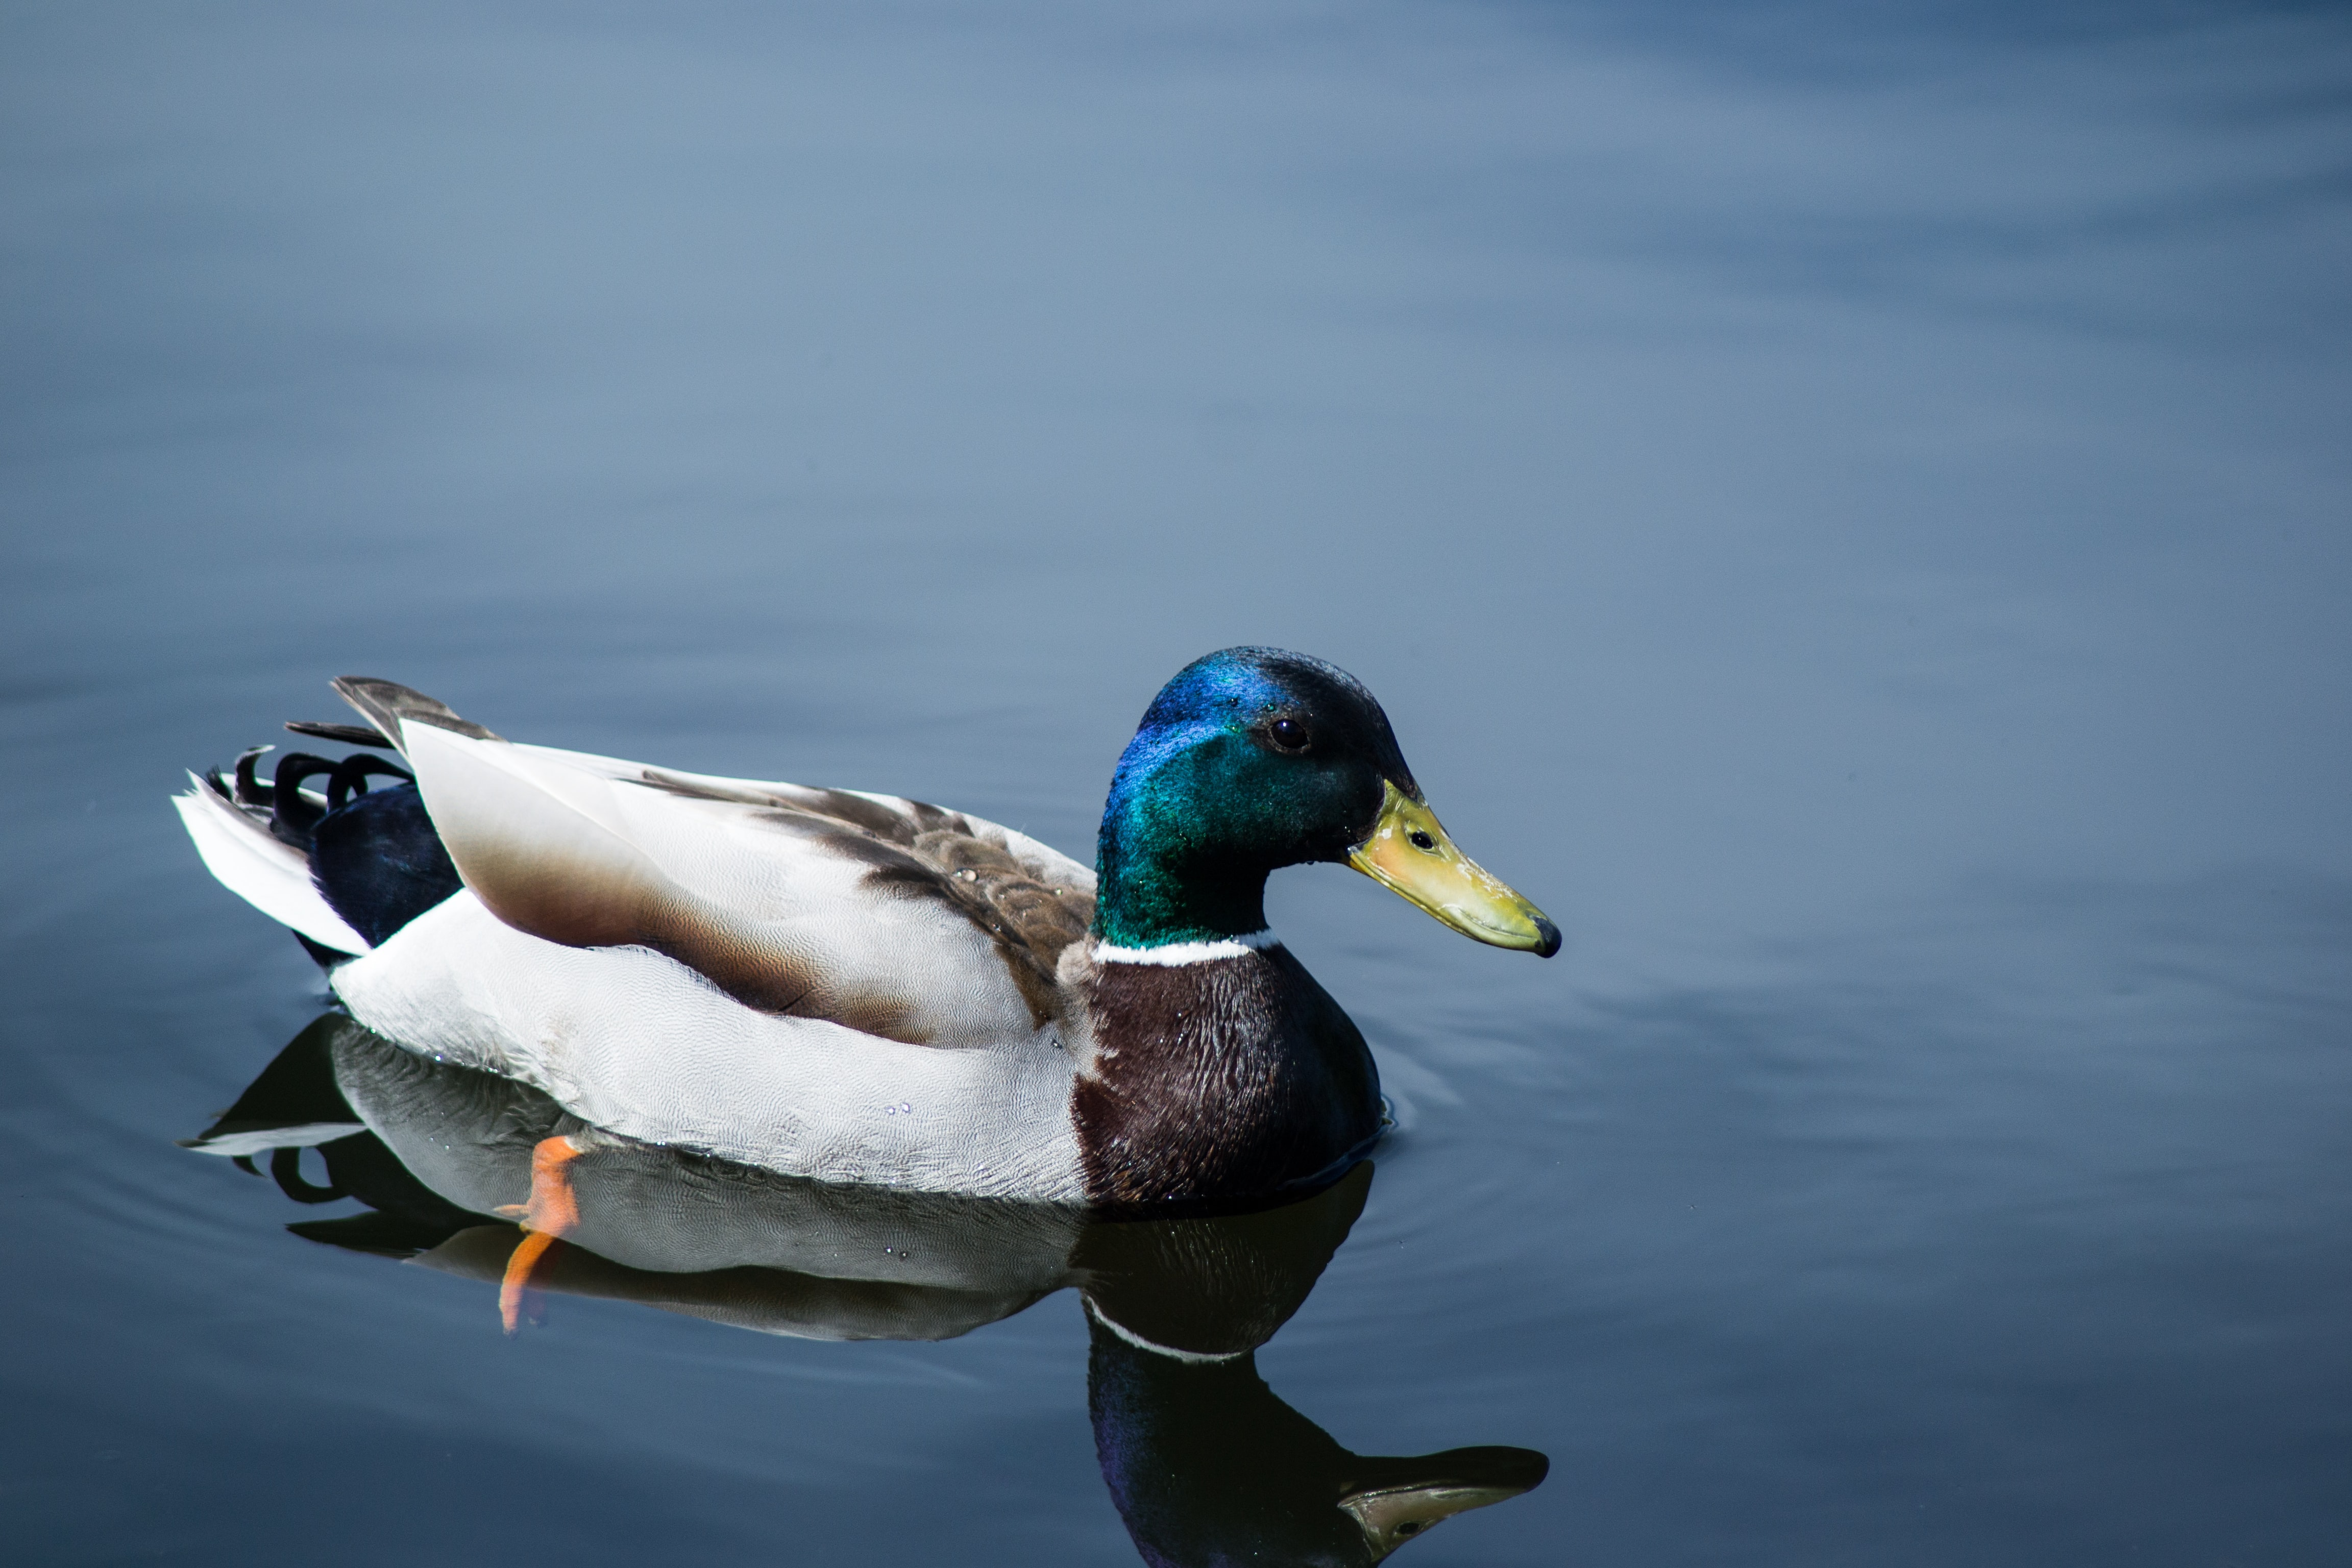
\includegraphics[width=\linewidth]{./Images/Chapter10/duck-hakon-helberg-unsplash.jpg}}%
{Håkon Helberg \href{https://unsplash.com/@hakonbrakon?utm_source=unsplash&utm_medium=referral&utm_content=creditCopyText}{Unsplash}}%
On voit qu'on se trouve dans une situation très différente de celle du programmeur C/C++, en ce sens que :
\begin{itemize}
	\item à l'écriture du programme, il n'y a aucun surcoût en matière de définition de type ;
	\item aucun contrôle de type n'est effectué \textit{a priori} par le langage au moment de la définition de la fonction \texttt{somme} ;
	\item par contre, au moment de l'exécution, s'il s'avère qu'on tente de faire une somme entre deux types qui ne peuvent pas être additionnés, comme ci-dessus avec un entier et une liste, le programme ne peut pas se dérouler correctement.
\end{itemize}

Au regard de la question du typage, deux points de vue coexistent :
\begin{enumerate}
	\item  les personnes habitués au typage statique se plaignent du typage dynamique en disant qu'on peut écrire des programmes faux et qu'on s'en rend compte trop tard, à l'exécution ;
	\item à l'inverse les partisans du typage dynamique font valoir que le typage statique est très partiel, par exemple, en C si on essaie d'écrire dans un pointeur \texttt{NULL}, le système d'exploitation ne le permet pas et le programme sort tout aussi brutalement.
\end{enumerate}

Selon l'approche, le typage dynamique est donc vécu comme inconvénient (pas assez de bonnes propriétés détectées par le langage) ou comme avantage (pas besoin de passer du temps à déclarer le type des variables, ni à faire des conversions pour satisfaire le compilateur).
Cependant, à l'usage, chacun peut constater qu'en matière de vitesse de développement, les inconvénients du typage dynamique sont très largement compensés par ses avantages.

\paragraph{Type {\normalfont\ttfamily hints}} Signalons enfin que depuis \textsc{Python\,3.5}, il est possible d'ajouter des annotations de type, pour expliciter les suppositions qui sont faites par le programmeur pour le bon fonctionnement du code.

Ces annotations sont totalement optionnelles et, même présentes, ne sont pas utilisées\sidenote{Ce point sera repris par la suite.} à l'exécution par l'interpréteur. L'idée est plutôt de permettre à des outils externes, à l'instar de \href{http://mypy-lang.org/}{\texttt{mypy}}, d'effectuer des contrôles plus poussés concernant la correction du programme.



%----------
\section[Types numériques]{Types numériques}
\label{sec:X.3}

\textsc{Python} offre quatre types d'objets numériques : les nombres entiers (\texttt{int}), décimaux (\texttt{float}), complexes (\texttt{complex}) et booléens (\texttt{bool}). Après leur présentation, certains aspects du calcul numérique sont évoqués.

\vspace{-6pt}
\subsection[Généralités]{Généralités}
\label{sub:X.3.1}


\subsubsection[Quatre types numériques]{Quatre types numériques}
\label{subsub:X.3.1.1}

Ouvrons un interpréteur \textsc{Python} et listons une à une les propriétés des différents types numériques.

%\vfill\pagebreak

\overparagraph{Nombre entier}

Pour créer un entier en \textsc{Python}, il suffit de le saisir dans l'interpréteur. Cependant, une fois la saisie validée, il n'y a aucun moyen de le manipuler car aucun nom lui a été attribué. Comme évoqué précédemment (cf. \cref{subsub:X.2.1.2}), il faut passer par le mécanisme de référencement et par exemple stipuler : \texttt{i = 1}. 
L'objet « \texttt{1} » est désormais référencé par la variable « \texttt{i} ».
\caution[t]<firstcolor>{%
Jusqu'à présent, de manière à ce qu'un nouvel utilisateur puisse y trouver ses marques, les environnements des différents interpréteurs \textsc{Python} ont été simulés tels que disponibles sur une plateforme \textsc{Ubuntu} MATE. Pour des raisons pratiques --- utilisation de l'extension \textsc{Python}\TeX\ --- et de lisibilité --- la coloration syntaxique sur fond noir est délicate ---, et contrairement aux illustrations du \textsc{Mooc}, ce n'est pas l'interpréteur \textsc{IPython} mais IDLE qui est dorénavant pris en exemple. Les différences sont minimes.}{Note de la rédaction}%
On peut s'assurer de son type au moyen de la fonction prédéfinie --- \textit{built-in} --- \texttt{type} (voir \cref{subsub:X.2.1.1}).

\vspace{4pt}% La présentation des \textit{notebooks} reste, quant à elle, inchangée.

\begin{ipythonminted}
§\ipythonuserprompt{user}{host}{~/programming}{\$}\textcolor{white}{ipython}§
§Python 3.8.2 (default, Apr 27 2020, 15:53:34)§
Type 'copyright', 'credits' §or§ 'license' §for§ more information
IPython §7.13.0§ -- An enhanced Interactive Python. Type '?' §for§ help.
§\ipythonpromptin{1}§ 1
§\ipythonpromptout{1}§ 1
§\ipythonpromptin{2}§ i = 1
§\ipythonpromptin{3}§ type(i)
§\ipythonpromptout{3}§ §int§
\end{ipythonminted}

\vspace{8pt}

%En \textsc{Python}, 

Les entiers se manipulent comme dans une calculatrice. Ainsi, on peut leur appliquer les quatre opérations de base que sont l'addition --- \texttt{1 + 4 = 5} ---, la soustraction --- \texttt{1 - 4 = -4} ---, la multiplication  --- \texttt{3 * 5 = 15} --- et la division  naturelle --- \texttt{3 / 6 = 0.5} ---, mais encore des fonctions plus élaborées comme les puissances --- \texttt{3 ** 3 = 27} --- ou la valeur absolue --- \texttt{abs(-4) = 4}.

\begin{idleshell*}[before skip=8pt, after skip=8pt]
Python 3.8.2 (default, Apr 27 2020, 15:53:34)\par
[GCC 9.3.0] on linux\par
Type "help", "copyright", "credits" or "license()" for more information.
\begin{pyconsole}
1
i = 1
type(i)
1 + 4
1 - 4
3 * 5
3 / 6
3 ** 3
abs(-4)
3 // 6
3 % 6
i = i + 5
print(i)
\end{pyconsole}
\end{idleshell*}

À noter qu'il existe aussi la division entière  --- \texttt{3 // 6 = 0} --- dont on obtient le reste avec l'opérateur modulo « \texttt{\%} » --- \texttt{3 \% 6 = 3}.

On peut bien entendu également réaffecter une variable avec le résultat d'une opération : \texttt{i = i + 5}, l'entier \texttt{i} vaut \texttt{1} donc \texttt{i + 5 = 6}. On peut le vérifier à l'aide de la fonction \textit{buit-in} \texttt{print} qui permet d'afficher le contenu\sidenote{À remarquer que l'on emploie soit la fonction \texttt{print()} ou le retour chariot. Ces deux fonctionnalités sont très proches et ne diffèrent de comportement que pour les chaînes de caractères. Cette différence est détaillée par la suite.} de la variable : \texttt{print(i) -> 6}.

%\begin{idleconsole}
%	\begin{pyconsole}
%		i = i + 5
%		print(i)
%	\end{pyconsole}
%\end{idleconsole}


%En \textsc{Python}, 

Les entiers ont la caractéristique remarquable d'être de précision illimitée. En affectant à la variable \texttt{i} un entier extrêmement grand, on peut le multiplier par lui même ou l’élever à la puissance \texttt{3} voire plus; on obtient toujours un entier sans aucune troncation de précision.

% i = 39457983745972375892347 597349285789347597349579
\begin{idleconsole}
	\begin{pyconsole}
		i = 39457983745972375892347
		i * i
		i ** 3
	\end{pyconsole}
\end{idleconsole}

\vspace{2pt}

\overparagraph{Nombre décimal}

Le type \texttt{float} est le deuxième type d'objet numérique en \textsc{Python}. Il est dévolu aux nombres décimaux. Primeur à l'anglais, le séparateur de décimales est le point, en lieu et place de la virgule en français.

Les décimaux ont une précision contrainte, généralement codés sur 15 chiffres significatifs et encodés sur 53 bits. Cela peut dépendre, évidemment, de la plateforme sur laquelle on fait tourner l'interpréteur.

\begin{idleconsole}
	\begin{pyconsole}
		f = 4.3
	\end{pyconsole}
\end{idleconsole}

\vspace{2pt}

\overparagraph{Nombre complexe}

Viennent ensuite les nombres complexes. Leur représentation est traditionnelle, en juxtaposant deux nombres décimaux, dont le second, pour la partie imaginaire, est suffixé par la lettre « \texttt{j} », ainsi : \texttt{4 + 5j}.

\begin{idleconsole}
	\begin{pyconsole}
		c = 4 + 5j
	\end{pyconsole}
\end{idleconsole}

\vspace{2pt}

\overparagraph{Conversion de type}

\textit{Stricto sensu}, \textsc{Python} se charge de toutes les conversions possibles. Bien entendu, il peut y avoir alors perte de précision.

L'addition d'un entier et d'un décimal donne un nombre décimal, avec perte de précision sur le nombre entier le cas échéant. En additionnant un entier, un décimal et un complexe, \textsc{Python} va fournir un complexe, toujours avec perte de précision si cela se présente.

La conversion d'un décimal vers un entier se réalise avec la fonction prédéfinie \texttt{int()} et va induire une troncation. À l'inverse la conversion d'un entier vers un décimal s'opère avec la fonction prédéfinie \texttt{float()}. Il en est de même pour les complexes avec \texttt{complex()}.

\begin{idleconsole}
	\begin{pyconsole}
		i = 39457983745972375892347597349285789347597349579
		f = 4.3
		i + f
		i + f + c
		int(4.3)
		float(4)
		complex(4.0)
	\end{pyconsole}
\end{idleconsole}
%		c = 4 + 5j

\vspace{2pt}

\overparagraph{Valeur booléenne}

Le dernier type numérique à présenter est celui des valeurs booléennes. En tant que tel, ce type est particulier car \textit{a priori} non censé faire partie des types numériques : valeur \texttt{True}/\texttt{False} pour vrai/faux. Bien noter que ces valeurs s'écrivent avec une première lettre capitale.

En \textsc{Python} comme quelques autres langages, le type booléen est codé en tant que sous-ensemble des entiers --- valeur \texttt{0} pour \texttt{False} et valeur \texttt{1} pour \texttt{True}. À titre d'illustration\sidenote{D'autres exemples d'application plus élaborés sont fournis par la suite.} est-que \texttt{1} est plus petit que \texttt{2} ? C'est vrai. Est-ce que \texttt{1} est plus grand que \texttt{5} ? c'est faux. 

\begin{idleconsole}
	\begin{pyconsole}
		1 < 2
		1 > 5
	\end{pyconsole}
\end{idleconsole}


\subsubsection[Manipulation comme calculette]{Manipulation comme calculette}
\label{subsub:X.3.1.2}

Au démarrage de l'interpréteur Python, on dispose en fait d'une calculette. Les \emph{règles de priorité} entre les différents opérateurs sont habituelles ; les produits et les divisions sont évalués en premier, ensuite les sommes et les soustractions.

\begin{linewidthnote}
De manière générale, il est recommandé de saisir des expressions correctement parenthésées. De plus, les parenthèses facilitent la lecture d'expressions complexes (cf. infra, la deuxième expression est équivalente de la troisième mais bien plus lisible).
\end{linewidthnote}

\sidetable[\label{tab:X.5}Opérateurs \textsc{Python}.]{%
\begingroup
\renewcommand*{\arraystretch}{1.6}
\rowcolors{2}{tableLineOne}{tableLineTwo}
\begin{tabularx}{\marginparwidth}{YX}
\rowcolor{secondcolor}
\multicolumn{2}{c}{\Gape[6pt]{\textcolor{white}{\textbf{Opérateurs en \textsc{Python}}}}} \\
\rowcolor{firstcolor}
\multicolumn{1}{c}{\scshape\titlingfont\textcolor{white}{Code}} 
	& \multicolumn{1}{c}{\scshape\titlingfont\textcolor{white}{Opération}} \\
\texttt{+}		& Addition \\
\texttt{-}		& Soustraction \\
\texttt{*}		& Multiplication \\
\texttt{/}		& Division \\
\texttt{//}		& Quotient \\
\texttt{\%}		& Modulo \\
\texttt{**}		& Puissance \\
\end{tabularx}%
\endgroup
}

\begin{idleshell}[before skip=8pt, after skip=8pt]
Python 3.8.2 (default, Apr 27 2020, 15:53:34)\par
[GCC 9.3.0] on linux\par
Type "help", "copyright", "credits" or "license()" for more information.
\vspace*{-.25\baselineskip}
\begin{pyconsole}
	20 * 60
	2 * 30 + 10 * 5
	(2 * 30) + (10 * 5)
	48 // 5  # calcul d'un quotient
	48 % 5   # modulo (reste de la division par)
	2 ** 10  # puissance
	(2 + 3j) * 2.5j  # multiplication de deux nombres complexes
	1j * 1.j
\end{pyconsole}
\end{idleshell}

On peut aussi facilement conduire des calculs sur les complexes. Se souvenir que la constante complexe marquée \texttt{i} en français se note \texttt{j} en \textsc{Python}, ce choix provient du BDFL\sidenote{\textit{Alias} Guido \textsc{van Rossum}.} pour des raisons de lisibilité.

Aussi, pour entrer ce nombre complexe \texttt{j}, il faut toujours le faire précéder d'un nombre, donc ne pas saisir simplement \texttt{j} (qui serait compris comme un nom de variable) mais plutôt \texttt{1j} ou encore \texttt{1.j}.

\paragraph{Variables} Il peut être utile de stocker un résultat qui sera utilisé plus tard ou de définir une valeur constante. Pour cela on utilise tout simplement une affectation.

\begin{idleconsole}[after skip=6pt]
	\begin{pyconsole}
	largeur = 5  # variable définie par assignation de valeur
	largeur * 20 # utilisation, ici comme un nombre
	largeur * 10 # après quoi bien sûr la variable reste inchangée
	\end{pyconsole}
\end{idleconsole}

Pour les symboles mathématiques, on peut utiliser la même technique. Pour les valeurs spéciales comme Π, on peut utiliser les valeurs prédéfinies par la bibliothèque mathématique de \textsc{Python}. En anticipant un peu sur la notion d'importation, on peut la charger et ainsi imprimer les racines troisièmes de l'unité\sidenote{Bien entendu, il sera possible de faire ceci plus simplement lorsque les boucles \texttt{for} seront vues.} par la formule :

\vspace*{-0.5\baselineskip}

\begin{equation}
r_n = e^{2i\pi \frac{n}{3}}, \mbox{ pour } n\in \{0,1,2\}
\end{equation}

\vspace*{0.225\baselineskip}

\begin{idleconsole}[after skip=7pt]
	\begin{pyconsole}
		pi = 3.14159  # réels : le point remplace la virgule du français
		2 * pi * 10
		from math import e, pi
		n = 0
		print("n=", n, "racine = ", e**((2.j*pi*n)/3))
		n = 1
		print("n=", n, "racine = ", e**((2.j*pi*n)/3))
		n = 2
		print("n=", n, "racine = ", e**((2.j*pi*n)/3))
	\end{pyconsole}
\end{idleconsole}

\paragraph{Types} Le changement par rapport à une calculatrice standard provient du fait que les valeurs soient typées. Illustration pour les trois types de nombres établis jusqu'ici.

\begin{idleconsole}[after skip=7pt]
	\begin{pyconsole}
		type(3)   # type entier : 'int'
		type(3.5) # type à virgule flottante : 'float'
		type(1j)  # type complexe : 'complex'
	\end{pyconsole}
\end{idleconsole}


\paragraph{Chaînes de caractères} On a également rapidement besoin de chaînes de caractères, étudiées par la suite en détail, mais en guise de mise en bouche, on peut écrire ce qui suit.

\begin{idleconsole}[after skip=7pt]
	\begin{pyconsole}
		chaine = "Bonjour le monde !"
		print(chaine)
	\end{pyconsole}
\end{idleconsole}

\paragraph{Conversions de type} Il est parfois nécessaire de convertir une donnée d'un type à un autre. Par exemple on peut demander à l'utilisateur d'entrer son âge au clavier grâce à la fonction \texttt{input}. 

Pour faire des calculs --- disons multiplier l'âge par deux ---, en s'y prenant naïvement, le résultat obtenu est surprenant ; il s'agit d'une concaténation de chaînes de caractères. En effet, la saisie à la volée s'opère assez logiquement sous le type chaîne de caractères. 
C'est pourquoi il faut ici d'abord convertir la (valeur de la) variable \texttt{reponse} en un entier, avant qu'il puisse ensuite être doublé (s'assurer au préalable de bien avoir entré une donnée qui corresponde à un nombre entier).

\begin{idleconsole}[after skip=6pt]
	\begin{pyverbatim}
		>>> reponse = input("quel est votre âge ? ")
	\end{pyverbatim}
	\vspace{-0.4\baselineskip}
	\textcolor{idleoutputcolor}{quel est votre âge ?}
	\begin{pycode}
		reponse = '35'
		print(reponse) # chaîne de caractère saisie
	\end{pycode}
	\vspace{-0.25\baselineskip}
	\pycon{reponse = '35'}
	\begin{pyconsole}
		print(reponse) # chaîne de caractère saisie
		type(reponse)  # variable de type chaîne de caractères
		2 * reponse    # multiplier une chaîne donne une concaténation
		age = int(reponse) # conversion de la chaîne en entier
		type(age)
		2 * age # désormais, on peut correctement multiplier par 2
		# ou le tout en une seule passe :
		print("le double de votre age est", 2*int(reponse))
	\end{pyconsole}
\end{idleconsole}

\sidetable[\label{tab:X.6}Fonction de typage \textsc{Python}.]{%
\begingroup
\renewcommand*{\arraystretch}{1.6}
\rowcolors{2}{tableLineOne}{tableLineTwo}
\begin{tabularx}{\marginparwidth}{XX}
\rowcolor{secondcolor}
\multicolumn{2}{c}{\Gape[6pt]{\textcolor{white}{\textbf{Fonction de typage en \textsc{Python}}}}} \\
\rowcolor{firstcolor}
\multicolumn{1}{c}{\scshape\titlingfont\textcolor{white}{Type}} 
	& \multicolumn{1}{c}{\scshape\titlingfont\textcolor{white}{Fonction}} \\
Entier		& \texttt{int} \\
Flottant		& \texttt{float} \\
Complexe		& \texttt{complex} \\
Chaîne		& \texttt{str} \\
\end{tabularx}%
\endgroup
}

De manière plus générale, pour convertir un objet en entier, en flottant ou en chaîne de caractères, on peut simplement appeler une fonction \textit{built-in} qui porte le même nom que le type cible (voir \cref{tab:X.6}). Ainsi dans l'exemple précédent, \texttt{int(reponse)} représente la conversion de \texttt{reponse} en entier.

\begin{idleconsole}
	\begin{pyconsole}
		a = 2345  # à l'inverse, si la donnée de départ est un entier
		str(2345) # conversion en chaîne de caractères
		complex(2345) # conversion en complexe
	\end{pyconsole}
\end{idleconsole}

Ceci se généralise à tous les types qui sont reconnus par \textsc{Python}, afin de convertir un objet \texttt{x} en un type \texttt{bidule}, on appelle \texttt{bidule(x)}.

\paragraph{Grands nombres} Comme les entiers sont de précision illimitée, on peut améliorer leur lisibilité en insérant des caractères \textit{underscore} « \texttt{\_} », lesquels sont simplement ignorés à l'exécution.

\begin{idleconsole}
	\begin{pyconsole}
		tres_grand_nombre = 23_456_789_012_345
		tres_grand_nombre
		123_456.789_012 # ça fonctionne aussi avec les flottants
	\end{pyconsole}
\end{idleconsole}

\vspace{1pt}

\paragraph{Entiers et bases} Les calculettes scientifiques permettent habituellement d'entrer les entiers dans d'autres bases que la base 10. En \textsc{Python}, on peut également saisir un entier sous forme binaire, octale (base 8) ou encore hexadécimale (base 16).

Pour d'autres bases, on peut utiliser la fonction de conversion \texttt{int} en lui passant un argument supplémentaire.

\begin{idleconsole}
	\begin{pyconsole}
		deux_cents = 0b11001000     # binaire
		deux_cents = 0o310          # octale
		deux_cents = 0xc8           # hexadécimale
		print(deux_cents)
		deux_cents = int('3020', 4) # quaternaire
		deux_cents = int('1300', 5) # quinaire
		print(deux_cents)
	\end{pyconsole}
\end{idleconsole}

\vspace{1pt}

\paragraph{Fonctions mathématiques} Naturellement, \textsc{Python} fournit un ensemble très complet d'opérateurs mathématiques pour les fonctions exponentielles, trigonométriques et autres. Cependant, à cette étape de la discussion, leur étude concrète est reportée à plus tard.

\subsubsection[Affectations et opérations]{Affectations et opérations (« à la \texttt{+=}) »}
\label{subsub:X.3.1.3}

Il existe en \textsc{Python} toute une famille d'opérateurs dérivés de l'affectation qui permettent de faire en une fois une opération et une affectation. En voici quelques morceaux choisis.

\paragraph{Incrémentation et autres} On peut facilement augmenter la valeur d'une variable numérique en employant \nopagebreak l'opérateur « \texttt{+=} ». 
Cette forme de directive, qui combine opération sur une variable et réaffectation du résultat à la même variable, est disponible avec tous les opérateurs courants (cf. \cref{tab:X.5}).

\begin{idleconsole}
	\begin{pyconsole}
		entier = 10
		entier += 2
		print('entier', entier)
		entier = 10  # équivalent aux lignes suivantes
		entier = entier + 2
		print('entier', entier)
		entier -= 4  # même syntaxe pour la soustraction
		print('après décrément', entier)
		entier *= 2  # même syntaxe pour la multiplication
		print('après doublement', entier)
		entier /= 2  # même syntaxe pour la division naturelle
		print('mis à moitié', entier)
		entier = 8
		entier /= 3  # même syntaxe pour la division entière
		print('mis à moitié', entier)
		entier = 2
		print('entier:', entier)
		entier **= 10
		print('à la puissance dix:', entier)
		entier %= 5
		print('modulo 5:', entier)
	\end{pyconsole}
\end{idleconsole}

\vspace{-1pt}

\paragraph{Types non numériques et opérateurs abscons} En réalité cette construction est disponible pour tous les types qui supportent l'opérateur employé. Par exemple, les listes (vues prochainement) peuvent être additionnées entre elles. 

Beaucoup de types supportent l'opérateur d'addition, qui est sans doute et de loin celui le plus utilisé avec cette construction. Signalons enfin que l'on trouve aussi cette construction avec d'autres opérateurs moins fréquents. Et pour ceux qui connaissent déjà un peu \textsc{Python}, on peut même l'appliquer avec des opérateurs de décalage.

\begin{idleconsole}
	\begin{pyconsole}
		liste = [0, 3, 5]
		print('liste', liste)
		liste += ['a', 'b']
		print('après ajout', liste)
		entier <<= 2
		print('double décalage gauche:', entier)
	\end{pyconsole}
\end{idleconsole}


\subsection[Compléments et application]{Compléments et application}
\label{sub:X.3.2}


\subsubsection[Précision des calculs flottants]{Précision des calculs flottants}
\label{subsub:X.3.2.1}

Comme pour les entiers, les calculs sur les nombres flottants sont réalisés par le processeur. 
Cependant, \nopagebreak contrairement au cas des entiers où les calculs sont toujours exacts, les flottants posent un problème de précision. Cela n'est pas propre au langage \textsc{Python}, mais dû à la technique de codage des nombres flottants sous forme binaire.

Il faut retenir que lorsqu'on écrit un nombre flottant sous forme décimale, la valeur utilisée en mémoire pour représenter ce nombre, parce que cette valeur est codée en binaire, ne représente \emph{pas toujours exactement} le nombre entré.

Aussi, les différentes erreurs d'arrondi qui se produisent à chaque étape du calcul s'accumulent et produisent un résultat parfois surprenant. De nouveau, ce problème n'est pas spécifique à \textsc{Python}, il existe pour tous les langages et il est bien connu\sidenote{En calcul scientifique --- simulation numérique, météorologie, etc. ---, ce point est crucial. En effet, de nombreuses itérations sont à produire en temps comme en espace. Il est alors impératif de pouvoir maîtriser ces erreurs d'arrondis, sans quoi les résultats sont aberrants.} des numériciens.

Dans une grande majorité des cas, ces erreurs d'arrondi ne sont pas pénalisantes. Il faut toutefois en être conscient car cela peut expliquer des comportements curieux.

\begin{idleconsole}
	\begin{pyconsole}
		0.2 + 0.4
		0.3 - 0.1 == 0.2  # expression fausse : erreur d'arrondi
	\end{pyconsole}
\end{idleconsole}

\vspace{1pt}

\overparagraph{Solution ? Penser en termes de nombres rationnels}

Si le problème se pose bien en termes de nombres rationnels, il est alors tout à fait possible de le résoudre avec exactitude.

Alors qu'il n'est pas possible d'écrire exactement 3/10 en base 2, ni d'ailleurs 1/3 en base 10, on peut représenter exactement ces nombres dès lors qu'on les considère comme des fractions et qu'on les encode avec deux nombres entiers.

\textsc{Python} fournit en standard le module \texttt{fractions} qui permet de résoudre le problème. Voici comment on pourrait l'employer pour vérifier --- cette fois avec succès ---, que \texttt{0.3 − 0.1} vaut bien \texttt{0.2}. Ce code anticipe sur l'utilisation des modules et des classes en \textsc{Python}, ici des objets de type \texttt{Fraction} sont créés.

\begin{idleconsole*}
	\begin{pyconsole}
		from fractions import Fraction  # import du module qui définit le symbole Fraction
		Fraction(3, 10) - Fraction(1, 10) == Fraction(2, 10)  # cette fois, calculs exacts
		Fraction('0.3') - Fraction('0.1') == Fraction('2/10')  # équivalent encore plus lisible
	\end{pyconsole}
\end{idleconsole*}

\vspace{1pt}

\overparagraph{Autre solution ? Module « {\normalfont\texttt{decimal}} »}

Si par ailleurs, pour quelconque raison, les nombres rationnels ne sont pas manipulés, du coup la représentation sous forme de fractions ne peut pas convenir. 

Indiquons alors l'existence du module standard \texttt{decimal} qui offre des fonctionnalités très voisines du type \texttt{float}, tout en éliminant la plupart des inconvénients, mais au prix, bien entendu, d'une consommation mémoire supérieure.

\begin{idleconsole}
	\begin{pyconsole}
		from decimal import Decimal
		Decimal('0.3') - Decimal('0.1') == Decimal('0.2')
	\end{pyconsole}
\end{idleconsole}

\begin{gofurther}
Tous les documents qui suivent sont en anglais :
\begin{itemize}\jazzitem
\item \href{https://docs.python.org/3/tutorial/floatingpoint.html}{tutoriel sur les nombres flottants} ;
\item \href{https://docs.python.org/3/library/fractions.html}{documentation sur la classe \texttt{Fraction}} ;
\item \href{https://docs.python.org/3/library/decimal.html}{documentation sur la classe \texttt{Decimal}} ;
%\item \href{http://ww5.oxfordmathcenter.com/drupal7/node>/43}{présentation détaillée sur l'encodage des flottants} (lien mort). Ce document, très bien fait, ne dépend pas du langage \textsc{Python} mais illustre le standard \textsc{IEE-754} sur des exemples concrets.
\end{itemize}
\end{gofurther}


\subsubsection[Opérations bit à bit (\textit{bitwise})]{Opérations bit à bit (\textit{bitwise})}
\label{subsub:X.3.2.2}

Il s'agit dans cette section d'expliquer des fonctions évoluées\sidenote{Sans souci, les débutants en programmation peuvent sauter cette partie en cas de difficulté.} sur les entiers. 
Outre les opérations déjà commentées, il est également possible de faire des opérations bit à bit sur les nombres entiers. 

Le plus simple est de penser à l'écriture du nombre en base 2.
Considérons par exemple deux entiers constants et leur transcription en binaire, comme par exemple :

\begin{idleconsole}[after skip=6pt]
	\begin{pyconsole}
		x49 = 49
		y81 = 81
	\end{pyconsole}
\end{idleconsole}

\begin{equation}
\begin{aligned}
x49 = 49 = 32 + 16 + 1 \rightarrow (0, 1, 1, 0, 0, 0, 1) \\
x81 = 81 = 64 + 16 + 1 \rightarrow (1, 0, 1, 0, 0, 0, 1)
\end{aligned}
\end{equation}

Pour comprendre comment passer de $32 + 16 + 1$ à $(0, 1, 1, 0, 0, 0, 1)$ et $64 + 16 + 1$ à $(1, 0, 1, 0, 0, 0, 1)$, il suffit d'observer que :

\vspace{-\baselineskip}
\begin{equation}
\begin{aligned}
32 + 16 + 1 = \mathbf{0}*2^6 + \mathbf{1}*2^5 + \mathbf{1}*2^4 + \mathbf{0}*2^3 + \mathbf{0}*2^2 + \mathbf{0}*2^1 +\mathbf{1}*2^0 \\
64 + 16 + 1 = \mathbf{1}*2^6 + \mathbf{0}*2^5 + \mathbf{1}*2^4 + \mathbf{0}*2^3 + \mathbf{0}*2^2 + \mathbf{0}*2^1 + \mathbf{1}*2^0 
\end{aligned}
\end{equation}

%\vspace{-0.2\baselineskip}

\overparagraph{Opérateurs logiques}

L'opération logique « \texttt{\&} » va faire un \textit{et} logique bit à bit entre les opérandes, ainsi :

\begin{idleconsole}
	\begin{pyconsole}
		x49 & y81
	\end{pyconsole}
\end{idleconsole}

En effet, on s'y retrouve car on a :

\vspace{-0.7\baselineskip}
\begin{equation}
\begin{array}{r@{~}c@{~}l}
x49 & \rightarrow & (0, 1, 1, 0, 0, 0, 1) \\
x81 & \rightarrow & (1, 0, 1, 0, 0, 0, 1) \\
x49\, \&\, y81 &\rightarrow & (0, 0, 1, 0, 0, 0, 1) \rightarrow 16 + 1 \rightarrow 17
\end{array}
\end{equation}

Ici, l'opérateur logique « \texttt{|} » fait simplement un \textit{ou} logique :

\begin{idleconsole}
	\begin{pyconsole}
		x49 | y81
	\end{pyconsole}
\end{idleconsole}

Cette fois, parce que :

\vspace{-0.7\baselineskip}
\begin{equation}
\begin{array}{r@{~}c@{~}l}
x49 & \rightarrow & (0, 1, 1, 0, 0, 0, 1) \\
x81 & \rightarrow & (1, 0, 1, 0, 0, 0, 1) \\
x49\, | \, y81 &\rightarrow & (1, 1, 1, 0, 0, 0, 1) \rightarrow 64 + 32 + 16 + 1 \rightarrow 113
\end{array}
\end{equation}

Enfin, on peut également conduire la même opération à base de \textit{ou exclusif} avec l'opérateur « \texttt{\^{}} » :

\begin{idleconsole}
	\begin{pyconsole}
		x49 ^ y81
	\end{pyconsole}
\end{idleconsole}

Le \textit{ou exclusif} de deux bits est vrai si et seulement si exactement une des deux entrées est vraie.

\vspace{-0.7\baselineskip}
\begin{equation}
\begin{array}{r@{~}c@{~}l}
x49 & \rightarrow & (0, 1, 1, 0, 0, 0, 1) \\
x81 & \rightarrow & (1, 0, 1, 0, 0, 0, 1) \\
x49\, \hat{} \, y81 &\rightarrow & (1, 1, 0, 0, 0, 0, 0) \rightarrow 64 + 32 \rightarrow 96
\end{array}
\end{equation}

\overparagraph{Décalages}

Un décalage à gauche de, par exemple quatre positions, revient à décaler tout le champ de bits de quatre cases à gauche (les quatre nouveaux bits insérés sont toujours des 0). C'est donc équivalent à une multiplication par $2^4 = 16$.

\begin{idleconsole}
	\begin{pyconsole}
		x49 << 4
	\end{pyconsole}
\end{idleconsole}

\vspace*{-1.2\baselineskip}

\begin{equation}
\begin{array}{r@{~}c@{~}l}
x49 & \rightarrow & (0, 1, 1, 0, 0, 0, 1) \\
x49\, << \, 4 &\rightarrow & (0, 1, 1, 0, 0, 0, 1, 0, 0, 0, 0) \rightarrow 512 + 256 + 16 \rightarrow 784
\end{array}
\end{equation}

De la même manière, le décalage à droite de $n$ revient à une division par $2n$ (plus précisément, le quotient de la division).

\begin{idleconsole}
	\begin{pyconsole}
		x49 >> 4
	\end{pyconsole}
\end{idleconsole}

%\vspace{-0.4\baselineskip}
\begin{equation}
\begin{array}{r@{~}c@{~}l}
x49 & \rightarrow & (0, 1, 1, 0, 0, 0, 1) \\
x49\, >> \, 4 &\rightarrow & (0, 0, 0, 0, 0, 1, 1) \rightarrow 2 + 1 \rightarrow 3
\end{array}
\end{equation}

\overparagraph{Astuce}

On peut utiliser\sidenote{Pour poursuivre l'exploration, consulter la documentation de \textsc{Python} :\\ \url{https://docs.python.org/3/library/stdtypes.html\#bitwise-operations-on-integer-types}} la fonction \textit{built-in} \texttt{bin} pour calculer la représentation binaire d'un entier. Attention, la valeur de retour est une chaîne de caractères de type \texttt{str}. Dans l'autre sens, on peut aussi saisir un entier directement en base $2$.

\begin{idleconsole}
	\begin{pyconsole}
		bin(x49)
		x49bis = 0b110001
		x49bis == x49
	\end{pyconsole}
\end{idleconsole}

Ici, \texttt{x49bis} est bien un entier.


\subsubsection[Exercices]{Exercices}
\label{subsub:X.3.2.3}

En corollaire de la discussion sur la précision des flottants, il faut savoir que le système de codage en mémoire impose aussi une limite. Les réels très petits ou très grands, ne peuvent plus être représentés de cette manière.

C'est notamment très gênant si on implémente un logiciel probabiliste --- comme des graphes de \textsc{Markov} --- où les probabilités d'occurrence de séquences très longues tendent très rapidement vers des valeurs extrêmement petites.


\begin{exercise}[title=Plus petit flottant, level=basic]
Le but de cet exercice est d'estimer la valeur du plus petit flottant qui peut être représenté comme un flottant. Pour aider, voici deux valeurs :
\begin{idleconsole}
	\begin{pyconsole}
		10**-320
		10**-330
	\end{pyconsole}
\end{idleconsole}

%\begin{nbjupyterin}[before skip=4pt, after skip=1pt]{1}
%10**-320
%\end{nbjupyterin}
%\begin{nbjupyterout}[before skip=1pt, after skip=4pt]{1}
%'abcdef'
%\end{nbjupyterout}
%\begin{nbjupyterin}[before skip=4pt, after skip=1pt]{2}
%10**-330
%\end{nbjupyterin}
%\begin{nbjupyterout}[before skip=1pt, after skip=4pt]{2}
%0.0
%\end{nbjupyterout}

Comme on le constate, $10^{−320}$ est correctement imprimé, alors que $10^{−330}$ est, de manière erronée, rapporté comme étant nul.

\noindent \lightbf{Remarques :}
\begin{itemize}\jazzitem
	\item À ce stade du cours, pour estimer le plus petit flottant, procéder simplement par approximations successives ;
	\item Sans utiliser de boucle, la précision obtenue n'est que fonction de la patience accordée à l'exercice par l'expérimentateur, ne dépasser pas 4 à 5 itérations successives ;)
	\item Il est par contre pertinent d'utiliser une approche rationnelle pour déterminer l'itération suivante (par opposition à une approche « au petit bonheur »). Pour ceux qui ne connaissent pas, il est recommandé de se documenter sur l'algorithme de \href{https://fr.wikipedia.org/wiki/Recherche\_dichotomique}{dichotomie} ;
	\item l'intérêt du \textit{notebook} par rapport à un document écrit est de pouvoir expérimenter directement dans le fil de l'énoncé (pour créer de nouvelles cellules saisir \keys{Alt+Enter}) ou, sinon, ouvrir un interpréteur comme IDLE.
\end{itemize}
\end{exercise}

\vfill
\pagebreak

\begin{exercise}[title=Plus grand flottant, level=basic]
La même limitation s'applique aux grands nombres. Toutefois, cela est un peu moins évident, car comme toujours il faut faire attention aux types.

En utilisant un exposant entier, les choses se passent bien. Dans ce premier cas \textsc{Python} calcule le résultat comme un \texttt{int}, qui est un type qui n'a pas de limitation de précision (\textsc{Python} utilise intelligemment autant de bits que nécessaire pour ce genre de calculs).

En revanche, si on essaie de conduire le même calcul avec un exposant flottant, on obtient une erreur.

\begin{idleconsole}% Pb de "breaklines" avec que des zéros (WHY?)
	\begin{pyverbatim}
		>>> 10**450
	\end{pyverbatim}
	\vspace{-0.4\baselineskip}
	\textcolor{idleoutputcolor}{1000000000000000000000000000000000000000000000000000000000000000}
	\textcolor{idleoutputcolor}{0000000000000000000000000000000000000000000000000000000000000000}
	\textcolor{idleoutputcolor}{0000000000000000000000000000000000000000000000000000000000000000}
	\textcolor{idleoutputcolor}{0000000000000000000000000000000000000000000000000000000000000000}
	\textcolor{idleoutputcolor}{0000000000000000000000000000000000000000000000000000000000000000}
	\textcolor{idleoutputcolor}{0000000000000000000000000000000000000000000000000000000000000000}
	\textcolor{idleoutputcolor}{0000000000000000000000000000000000000000000000000000000000000000}
	\textcolor{idleoutputcolor}{000000000000000000000000000000000000000000000000}
	\begin{pyconsole}[][breaklines, breakafter=0123456789]
		10**450.0
	\end{pyconsole}
\end{idleconsole}

On peut d'ailleurs remarquer que le comportement n'est pas vraiment cohérent, car avec les petits nombres \textsc{Python} a silencieusement transformé $10^{−330}$ en $0$, alors que pour les grands nombres, il lève une exception.

Quoi qu'il en soit, la limite pour les grands nombres se situe entre les deux valeurs $10^300$ et $10^310$. On demande à nouveau d'estimer comme ci-dessus une valeur approchée du plus grand nombre possible de représenter comme un flottant.

\begin{idleconsole}
	\begin{pyconsole}
		10**300.
		10**310.
	\end{pyconsole}
\end{idleconsole}
\end{exercise}

%\vspace{-4pt}

\overparagraph*{Compléments avancés} 

En fait, on peut accéder aux valeurs minimales et maximales des flottants au moyen du module \texttt{sys}, pour « \textit{system} » ; en particulier avec la \href{https://docs.python.org/3/library/sys.html\#sys.float\_info}{méthode \texttt{float\_info}}.

\emph{Sauf que} si le maximum observé expérimentalement est voisin de cette valeur, le minimum ne correspond pas bien à celui donné par le module \texttt{sys}. L'explication de cette apparente contradiction réside dans l'utilisation de « \href{https://en.wikipedia.org/wiki/Denormal\%5Fnumber}{nombres \emph{dénormaux}} ».

\begin{idleconsole}
	\begin{pyconsole}[][breaklines, breakafter=0123456789]
		import sys
		print(sys.float_info)
		print("Flottant minimum", sys.float_info.min)
		print("Flottant maximum", sys.float_info.max)
	\end{pyconsole}
\end{idleconsole}

\vfill\pagebreak

%----------
\section[Que faire de ces ressources ? Quiz]{Que faire de ces ressources ? Autoévaluation}
\label{sec:X.4}

%\subsubsection[Autoévaluation]{Autoévaluation}
%\label{subsub:X.3.2.4}

Le questionnaire\caution[t]<firstcolor>{%
La présentation des quiz du document\linebreak suit plus ou moins celle de la platefor\-me \textsc{Fun-Mooc}. La fonctionnalité manquante --- pas encore implémentée dans l'extension de style \LaTeX{} usitée --- est relative à la comptabilisation des points et à leur enregistrement. Aussi, il appartient au lecteur de jouer le jeu dans l'auto\-évaluation de ses connaissances.}{Note de la rédaction}
à choix multiple%
\parnote{De manière traditionnelle en \textsc{Ihm}, lorsqu'une seule réponse est correcte, les propositions sont précédées d'un cercle à cocher (\emph{radio button}) ; en revanche, dans le cas de plusieurs solutions possibles, il s'agit de carrés (\emph{check box}). En outre, après validation des réponses (« Vérifier »), leur explication s'affiche en marge ou infobulle (« Afficher la réponse »).}
--- QCM --- à suivre porte sur le présent chapitre \qnameref{chap:X}.
\parnotes

\vspace*{6pt}


\begin{quiz}[title={Variable, objet et typage dynamique}]
\vspace{-\baselineskip}
\begin{quizquestion}[t]{2,4}{1,3}{Objets, affectation, typage dynamique}
<En \textsc{Python}, seuls les objets ont un type, les variables n'ont pas de type et c'est le mécanisme de typage dynamique qui permet d'associer un objet (typé) à une variable (sans type).\\
\textsc{Python} emploie le typage dynamique mais aussi le typage fort. Ce sont deux notions à ne pas confondre. Avec le typage fort, tous les objets ont un type et celui-ci ne peut plus changer après la création de l'objet.
En revanche, une variable ne définit qu'un nom pour un objet ; on peut la réaffecter plus tard à un objet d'un autre type.>
\points{1}
Quelles affirmations sont vraies ?
	\mcqproposal{Chaque variable possède un type.}
	\mcqproposal{Chaque objet possède un type.}
	\mcqproposal{Le typage dynamique permet de changer le type des objets.}
	\mcqproposal{L'opération d'affectation donne un nom à un objet.}
\end{quizquestion}

\begin{quizquestion}[c]{1,3,5,7}{2,4,6}{Noms de variable}
<\begin{jazzitemize}
	\item La réponse 2 est fausse car le caractère « \texttt{-} » n'est pas autorisé.
	\item La réponse 4 est erronée car le caractère « \texttt{:} » n'est pas autorisé.
	\item La réponse 6 est également mauvaise car un identifiant ne peut pas commencer par un chiffre.
\end{jazzitemize}
Les autres réponses sont correctes.>
\points{1}
%Parmi les noms de variables suivants, lesquels sont autorisés par le langage \textsc{Python} ? %Plusieurs réponses sont possibles.\\
%Pour être clair, on parle bien de ce qui est permis par le langage, sans tenir compte de ce qui est recommandé ou non.
Quels sont les noms de variables suivants autorisés\parnote{Pour être très clair, on parle bien de ce qui est permis par le langage, sans tenir compte de ce qui est recommandé ou non.} en \textsc{Python} ?
\parnotes
	\mcqproposal{\texttt{nom\_de\_variable}}
	\mcqproposal{\texttt{nom-de-variable}}
	\mcqproposal{\texttt{nom\_de\_variable2}}
	\mcqproposal{\texttt{nom:de:variable}}
	\mcqproposal{\texttt{NomDeVariable}}
	\mcqproposal{\texttt{2eme\_variable}}
	\mcqproposal{\texttt{\_nom\_de\_variable}}
\end{quizquestion}

\begin{quizquestion}[b]{2,4}{1,3}{Mots-clefs}
<\begin{jazzitemize}
	\item \texttt{var} est légal, ce n'est pas un mot-clé en \textsc{Python}.
	\item \texttt{if} et \texttt{True} sont des mots-clés, on ne peut pas les utiliser comme nom de variable.
\end{jazzitemize}
En revanche, \texttt{true} est une variable possible, car les noms de variables sont sensibles à la casse ; ce n'est naturellement pas une pratique recommandée.
De même, on peut en théorie utiliser les accents français, cédilles et caractères de l'alphabet grec, même si cette pratique est déconseillée.>
\points{1}
%Parmi les noms de variables suivants, lesquels sont autorisés par le langage \textsc{Python} ?
Quels sont les noms de variables suivants autorisés en \textsc{Python} ?
	\mcqproposal{\texttt{var}}
	\mcqproposal{\texttt{if}}
	\mcqproposal{\texttt{True}}
	\mcqproposal{\texttt{true}}
	\mcqproposal{\texttt{prénom\_garçon}}
	\mcqproposal{β\texttt{1}}
\end{quizquestion}
\end{quiz}


\begin{quiz}[title={Type numériques}]
\vspace{-\baselineskip}
\begin{quizquestion}[b]{1,4}{2,3}{Calcul de puissances}
<L'opérateur de puissance est « \texttt{**} » en \textsc{Python}. 
On peut obtenir aussi le résultat en partant de 1 (un seul bit), avec un décalage à gauche de 16 bits.>
Comment calculer la 16\textsuperscript{ième} puissance de 2 ? %Rappel : plusieurs réponses sont possibles.
\points{1}
	\mcqproposal{\pyv{2 ** 16}}
	\mcqproposal{\pyv{2 && 16}}
	\mcqproposal{\pyv{2 | 16}}
	\mcqproposal{\pyv{1 << 16}}
\end{quizquestion}

\begin{quizquestion}[b]{4,5}{1,2,3,6}{Nombres flottants}
<L'opérateur « \texttt{/} » est la division en \textsc{Python}, les trois premières expressions s'évaluent toutes à \texttt{1.2}.
La dernière expression est une opération entre entiers, elle retourne donc l'entier 1 et un entier n'est pas un flottant.>
\points{1}
Parmi les expressions suivantes, quelles sont celles qui retournent un flottant dont la valeur est $1.0$ ?
	\mcqproposal{\pyv{(3.0 + 3.0) / 5 }}
	\mcqproposal{\pyv{(3.0 + 3) / 5}}
	\mcqproposal{\pyv{(3 + 3) / 5}}
	\mcqproposal{\pyv{(3.0 + 3.0) // 5}}
	\mcqproposal{\pyv{(3.0 + 3) // 5}}
	\mcqproposal{\pyv{(3 + 3) // 5}}
\end{quizquestion}

\begin{quizquestion}[b]{2,3,4,5}{1,6,7}{Nombres complexes}
<\textsc{Python} utilise « \texttt{j} » plutôt que « \texttt{i} » pour identifier la partie imaginaire.
Les deux dernières formes font référence à une variable « normale » qui appellerait « \texttt{i} » ou « \texttt{j} »'>
\points{1}
Comment saisir au clavier la valeur du complexe \texttt{3 + 2i} ?
	\mcqproposal{\pyv{3 + 2i}}
	\mcqproposal{\pyv{3 + 2j}}
	\mcqproposal{\pyv{3 + 2 * 1j}}
	\mcqproposal{\pyv{3 + 2 * 1.j}}
	\mcqproposal{\pyv{3 + 2.j}}
	\mcqproposal{\pyv{3 + 2 * i}}
	\mcqproposal{\pyv{3 + 2 * j}}
\end{quizquestion}
\end{quiz}


%\vspace*{2.0\baselineskip}
%\begin{center}
%\pgfornament[width=0.3333\linewidth, color=secondcolor]{75}
%\end{center}

\vfill\pagebreak\thispagestyle{empty}






